\documentclass[a4paper,12pt]{scrreprt}
\usepackage[utf8]{inputenc}
\usepackage[provide=*,german]{babel}
\usepackage[T1]{fontenc}
\usepackage{amsmath}
\usepackage{amssymb}
\usepackage{amsthm}
\usepackage{mathtools}
\usepackage{geometry}
\usepackage{graphicx}
\usepackage[hidelinks]{hyperref}
\usepackage{listings}
\usepackage{xcolor}
\usepackage{algorithm}
\usepackage{algpseudocode}
\usepackage{chngcntr}
\usepackage{tikz}
\usepackage{float}
\usepackage{booktabs}
\usepackage{caption}
\usepackage{subcaption}
\usepackage{pgfplots}
\usepackage{microtype}
\usepackage{array}
\usepackage{rotating}
\usepackage{etoolbox}
\usepackage{enumitem}
\usepackage{braket}
\usepackage{multirow}
\usepackage{siunitx}
\usepackage{bm}

\setlist[itemize,1]{label=-}

\usetikzlibrary{positioning,shapes,arrows,shadows,calc,automata,
  arrows.meta, shapes.geometric, decorations.pathmorphing,
  patterns, decorations.markings, fit, backgrounds}
\pgfplotsset{compat=1.18}
\geometry{margin=2.5cm}

% ------------------------------------------------------------------
% section als oberste Ebene, ab 1, kein chapter-Präfix
% ------------------------------------------------------------------
\counterwithout{section}{chapter}
\renewcommand{\thesection}{\arabic{section}}

\RedeclareSectionCommand[
  beforeskip=2\baselineskip,
  afterskip=1\baselineskip,
  font=\Large\bfseries
]{section}
\RedeclareSectionCommand[
  beforeskip=1\baselineskip,
  afterskip=0.5\baselineskip
]{subsection}
\RedeclareSectionCommand[
  beforeskip=0.75\baselineskip,
  afterskip=0.25\baselineskip
]{subsubsection}
\RedeclareSectionCommand[
  beforeskip=0.5\baselineskip,
  afterskip=-1em,
  font=\normalfont\bfseries
]{paragraph}

\DeclareTOCStyleEntry[
  indent=0pt,
  numwidth=2em,
  entryformat=\bfseries,
  pagenumberformat=\bfseries,
  beforeskip=0.5em
]{tocline}{section}

% ------------------------------------------------------------------
% Theorem-Umgebungen
% ------------------------------------------------------------------
\theoremstyle{definition}
\newtheorem{definition}{Definition}[section]
\newtheorem{bemerkung}{Bemerkung}[section]
\newtheorem{beispiel}{Beispiel}[section]
\newtheorem{satz}{Satz}[section]
\newtheorem{lemma}{Lemma}[section]
\newtheorem{korollar}{Korollar}[section]
\newtheorem{frage}{Frage}[section]
\newtheorem{proposition}{Proposition}[section]

\counterwithin{algorithm}{section}
\counterwithin{figure}{section}
\counterwithin{table}{section}

\counterwithout{equation}{chapter}

\hypersetup{
	colorlinks=true,
	linkcolor=blue!60!black,
	urlcolor=blue!60!black,
	citecolor=blue!60!black
}

\lstset{
  basicstyle=\ttfamily\footnotesize,
  breaklines=true,
  frame=single,
  numbers=left,
  numberstyle=\tiny\color{gray},
  keywordstyle=\color{blue}\bfseries,
  commentstyle=\color{green!60!black},
  stringstyle=\color{red},
  showstringspaces=false,
  tabsize=4,
  captionpos=b,
  literate={ä}{{\"a}}1 {ö}{{\"o}}1 {ü}{{\"u}}1
           {Ä}{{\"A}}1 {Ö}{{\"O}}1 {Ü}{{\"U}}1
           {ß}{{\ss}}1
}

%% Makros
\newcommand{\kb}{k_\mathrm{B}}
\newcommand{\hc}{\hbar c}
\newcommand{\neff}{n_\mathrm{eff}}
\newcommand{\dquer}{\bar{d}}
\newcommand{\Tcoh}{T_\mathrm{coh}}
\newcommand{\ordre}[1]{\mathcal{O}\!\left(#1\right)}
\newcommand{\Realteil}{\operatorname{Re}}
\newcommand{\Imagteil}{\operatorname{Im}}
\newcommand{\Tr}{\operatorname{Tr}}
\DeclareMathOperator{\sgn}{sgn}
\newcommand{\vect}[1]{\bm{#1}}
\newcommand{\matr}[1]{\mathbf{#1}}

\pretocmd{\section}{\clearpage}{}{}
\captionsetup{format=plain, indention=0pt, hangindent=0pt}

\title{\textbf{Effiziente Nanostrukturen mit\\ Wasser und Licht}\\[0.8ex]
  \large Ionotronisches Flüssigkeits-Rechnen und photonische Oberflächen\\
  als neue Technologieplattformen adaptiver Nanomaterialien}
\author{Stephan Epp}
\date{27. Februar 2026}

\begin{document}

\maketitle
\tableofcontents
\newpage

% ===================================================================
\section{Einleitung und wissenschaftliche Vision}
% ===================================================================

\subsection{Zwei Paradigmen -- eine Konvergenz}

Die Geschichte der Mikro- und Nanotechnologie ist eine Geschichte der
Miniaturisierung fester, photolithographisch erzeugter Strukturen. Seit
Gordon Moore 1965 die empirische Beobachtung formulierte, dass sich die
Anzahl der Transistoren auf einem integrierten Schaltkreis ungefähr alle
zwei Jahre verdoppelt~\cite{moore1965}, haben Halbleiterhersteller dieses
Gesetz als Leitbild verfolgt. Gleichzeitig hat die Nanooptik in den
vergangenen Jahrzehnten gezeigt, dass Licht durch nanoskalige Strukturierung
von Oberflächen präzise geformt, gefärbt und dynamisch moduliert werden kann.

Die vorliegende Arbeit vereint zwei scheinbar getrennte Forschungsrichtungen
unter einem gemeinsamen Dach: das \textbf{Ionotronic Reconfigurable Fabric}
(IRF) -- ein wasserbasiertes, dynamisch rekonfigurierbares Berechnungsmedium
-- und die \textbf{aktive Nanooptik} durch programmierbare photonische
Oberflächen aus weichen Polymersystemen. Der verbindende Faden zwischen
beiden Feldern ist nicht zufällig: In beiden Fällen übernimmt ein flüssiges
oder quasiflüssiges Medium (Wasser, gequollenes Hydrogel) eine aktive
Funktionsrolle, die weit über die passive Trägersubstanz hinausgeht.

\textbf{Im ionotronischen Paradigma} übernimmt ein hochleitfähiges, ionisch
dotiertes Wasservolumen gleichzeitig drei Funktionen, die in klassischen
CMOS-Architekturen durch separate, fest verdrahtete Strukturen realisiert
werden müssen: Leitung, Schaltung und Speicherung. Diese dreifache
Simultaneität -- kurz \emph{Tripleximät} -- ist der entscheidende Vorteil,
der das IRF-Konzept von allen bisherigen Alternativen zu CMOS unterscheidet.

\textbf{Im nanooptischen Paradigma} ermöglicht die Quellungsdynamik eines
vernetzten Polymernetzwerks die kontinuierliche Durchstimmbarkeit eines
Fabry-P{\'e}rot-Resonators über das gesamte sichtbare Spektrum von
$\SI{420}{nm}$ bis $\SI{700}{nm}$. Durch Elektronenstrahlbestrahlung lassen
sich räumlich kodierte Quellungsgradienten erzeugen, die bei Kontakt mit
Wasser oder organischen Lösungsmitteln vordefinierte Topographien und
Farben offenbaren -- eine direkte technische Analogie zur dynamischen
Tarnung von Cephalopoden.

Die Konvergenz beider Paradigmen eröffnet eine neue Klasse von
\textbf{hydro-photonischen Nanoplattformen}: Systeme, in denen Wasser und
Licht gemeinsam als aktive Funktionsmedien agieren, um Information zu
verarbeiten, zu speichern, anzuzeigen und auf die Umgebung zu reagieren.

\subsection{Motivation und gesellschaftliche Relevanz}

Der weltweite Energieverbrauch von Rechenzentren übersteigt heute zwei Prozent
des globalen Stromverbrauchs und wächst mit der Verbreitung von Künstlicher
Intelligenz exponentiell~\cite{iea2023}. Der dominante Anteil dieser Energie
wird nicht für die eigentliche Informationsverarbeitung aufgewendet, sondern
für die Kühlung -- eine direkte Konsequenz der unvermeidlichen ohmschen
Verlustleistung in Halbleiterschaltern. Das IRF-Konzept adressiert dieses
Problem fundamental: Die Schaltenergie dissiiert nicht als Wärme im Festkörper,
sondern verformt Oberflächenspannungsenergie -- ein inhärent effizienterer
und lokal besser kontrollierbarer Mechanismus.

Gleichzeitig entstehen in der Photonik, der Sensorik und der adaptiven Optik
wachsende Anforderungen an Oberflächen, die ihr visuelles Erscheinungsbild
dynamisch anpassen können -- für adaptive Tarnung, biomedizinische
Sensordisplays, holographische Datenspeicherung und programmierbare
Metamaterialoberflächen. Die aktive Nanooptik mit weichen Polymersystemen
bietet hier eine biologisch inspirierte, energieeffiziente und kostengünstig
herstellbare Lösung.

Beide Technologieplattformen teilen eine strategische Eigenschaft: Sie erfordern
keine Extreme-UV-Lithographie und keine Milliarden-Investitionen in Reinraum-
infrastruktur wie TSMC-Fertigungsanlagen. Dies eröffnet ein reelles Fenster für
neue Marktteilnehmer und für die Neupositionierung der europäischen und deutschen
Technologieindustrie durch disruptive Innovation.

\subsection{Schlüsselbegriffe und Abkürzungen}

\textbf{Ionotronic Reconfigurable Fabric (IRF):} Wasserbasiertes,
rekonfigurierbares Berechnungsmedium auf Basis des EWOD-Prinzips.

\textbf{IoFET:} Ionotronic Field-Effect Transistor -- das wasserbasierte
Äquivalent zum MOSFET.

\textbf{EWOD:} Electrowetting-on-Dielectric -- elektrostatische Steuerung
des Benetzungswinkels.

\textbf{Fabry-P{\'e}rot-Resonator (FP):} Optischer Resonator aus zwei
halbdurchlässigen Spiegeln; zentrales Element der aktiven Farbsteuerung.

\textbf{TMM:} Transfermatrix-Methode -- systematisches Verfahren zur
Berechnung optischer Eigenschaften geschichteter Medien.

\textbf{Flory-Rehner-Modell:} Thermodynamisches Modell zur Beschreibung
der Quellung vernetzter Polymernetzwerke.

\textbf{Quellung (Swelling Ratio) $Q$:} Verhältnis gequollenes zu
trockenes Volumen eines Polymernetzwerks.

\textbf{Tripleximät:} Die simultane Funktion eines Wasservolumens als
Leiter, Schalter und Speicher (Begriff aus iono.tex).

\subsection{Aufbau der Arbeit}

Die Arbeit ist in 17 Kapitel gegliedert. Kapitel~2 behandelt
die gemeinsamen physikalischen Grundlagen beider Felder: ionische Leitung,
Elektrowetting, Oberflächenspannung und Nanooptik. Kapitel~3 stellt die
dreifache Simultaneität des IRF-Systems dar. Kapitel~4 beschreibt den IoFET.
Kapitel~5 entwickelt die Tropfenlogik. Kapitel~6 behandelt den
Fabry-P{\'e}rot-Resonator als Farbfilter. Kapitel~7 entwickelt die
Transfermatrix-Methode. Kapitel~8 beschreibt das Flory-Rehner-Quellungsmodell.
Kapitel~9 behandelt die Elektronenstrahl-Texturprogrammierung. Kapitel~10
formuliert das inverse Optimierungsproblem für photonische Strukturen. Kapitel~11 betrachtet die biologische Inspiration. Kapitel~12 analysiert die Konvergenz beider Plattformen und Synergien.
Kapitel~13 betrachtet die Transistordichte und Energiebilanz. Kapitel~14 zeigt Anwendungen. Kapitel~15 beschreibt die experimentelle Validierung. Kapitel~16 geht auf Grenzen und offene Fragen ein. Kapitel~17 fasst zusammen und gibt einen Ausblick.

% ===================================================================
\section{Physikalische Grundlagen}
% ===================================================================

\subsection{Wasser als multifunktionales aktives Medium}

Reines Wasser hat eine elektrische Leitfähigkeit von lediglich
$\sigma \approx 5{,}5 \times 10^{-6}$\,S/m bei $25\,^{\circ}C$ -- und ist damit
paradoxerweise gerade \emph{deshalb} interessant: Die Leitfähigkeit ist
über viele Größenordnungen präzise einstellbar, indem ionische Substanzen in
kontrollierter Konzentration gelöst werden.

\begin{definition}[Ionische Leitfähigkeit]
  Die elektrische Leitfähigkeit einer wässrigen Ionenlösung ist:
  \begin{equation}
    \sigma = \sum_i z_i \mu_i c_i F
    \label{eq:leitfaehigkeit}
  \end{equation}
  wobei $z_i$ die Wertigkeit, $\mu_i$ die Beweglichkeit, $c_i$ die molare
  Konzentration des $i$-ten Ionentyps und $F$ die Faraday-Konstante bezeichnet.
\end{definition}

Für die IRF-Technologie werden konzentrierte Kaliumchlorid-Lösungen
(KCl, $c \approx 0{,}1$ bis $1{,}0$\,mol/l) verwendet, die eine Leitfähigkeit
von $\sigma = 1$ bis $10$\,S/m erreichen. In der nanooptischen Anwendung
dient Wasser und verschiedene organische Lösungsmittel als Quellungsmedium
für Hydrogele, wobei der Quellungsgrad $Q$ die optischen Eigenschaften
(Schichtdicke $d$, Brechungsindex $n$) des Resonators bestimmt.

\paragraph{Wasser als optisches Medium.}
Wasser besitzt in weiten Bereichen des sichtbaren Spektrums einen
Brechungsindex von $n_\text{H$_2$O} \approx 1{,}33$ und ist nahezu
absorptionsfrei. Hydrogele mit eingelagertem Wasser haben Brechungsindizes
typischerweise im Bereich $n \approx 1{,}33$--$1{,}50$, je nach Polymergehalt.
Die Lorentz-Lorenz-Relation verknüpft den Brechungsindex mit der
Moleküldichte $N$:
\begin{equation}
  \frac{n^2 - 1}{n^2 + 2} = \frac{N \alpha}{3\varepsilon_0},
\end{equation}
wobei $\alpha$ die molekulare Polarisierbarkeit ist. Für ein gequollenes
Polymernetzwerk ändert sich $N$ mit dem Quellungsgrad $Q = V_\text{gequollen}/V_\text{trocken}$:
\begin{equation}
  N(Q) = \frac{N_0}{Q},
  \label{eq:dichte-quellung}
\end{equation}
was in erster Näherung zur linearen Relation
\begin{equation}
  n(Q) \approx 1 + \frac{n_0 - 1}{Q}
  \label{eq:n-quellung}
\end{equation}
führt, die für $Q \lesssim 5$ auf besser als $1\%$ genau ist.

\subsection{Ionentransport und Elektrokinetik}

Der Ladungstransport in ionischen Lösungen unterscheidet sich fundamental
von der Elektronen-Lochleitung in Halbleitern. Drei Transportmechanismen
wirken zusammen:

\paragraph{Elektromigration.}
Unter dem Einfluss eines elektrischen Feldes $\vec{E}$ bewegen sich Ionen
mit der Driftgeschwindigkeit $v_d = \mu_i \vec{E}$. Bei KCl beträgt die
Beweglichkeit von K$^+$ etwa $7{,}62 \times 10^{-8}$\,m$^2$/(V$\cdot$s)
und von Cl$^-$ etwa $7{,}91 \times 10^{-8}$\,m$^2$/(V$\cdot$s) -- eine
bemerkenswert ausgeglichene Paarung, die Konzentrationsgradienten
minimiert~\cite{atkins2018}.

\paragraph{Diffusion.}
Dem Fickschen Gesetz folgend transportiert thermische Bewegung Ionen aus
Bereichen hoher in Bereiche niedriger Konzentration. Der Diffusionskoeffizient
ist über die Einstein-Stokes-Relation verknüpft:
\begin{equation}
  D_i = \frac{\mu_i k_B T}{z_i e}.
  \label{eq:einstein_stokes}
\end{equation}

\paragraph{Elektroosmose.}
Nahe geladenen Oberflächen bildet sich eine elektrische Doppelschicht aus.
Ein anliegendes tangentiales elektrisches Feld treibt die Flüssigkeit als
Ganzes -- die Elektroosmose -- und erlaubt Flüssigkeitstransport ohne
mechanische Pumpen.

\subsection{Oberflächenspannung und Benetzungsphysik}

Die Oberflächenspannung von Wasser ($\gamma \approx 72$\,mN/m bei $25\,^{\circ}C$)
ist eine der höchsten aller bekannten Flüssigkeiten -- ein direktes Resultat
starker Wasserstoffbrückenbindungen.

\begin{satz}[Tropfenverschmelzung als Energieminimierung]
  Zwei Wassertropfen mit Radien $r_1$ und $r_2$ verschmelzen spontan, sofern:
  \begin{equation}
    4\pi\gamma(r_1^2 + r_2^2) > 4\pi\gamma(r_1^3 + r_2^3)^{2/3}.
    \label{eq:energieminimierung}
  \end{equation}
  Diese Bedingung ist für alle $r_1, r_2 > 0$ erfüllt.
\end{satz}

\subsection{Elektrowetting-on-Dielectric (EWOD)}

Das EWOD-Prinzip ist der zentrale Steuerungsmechanismus des IRF-Konzepts.
Es ermöglicht, den Kontaktwinkel $\theta$ eines Wassertropfens durch eine
anliegende Spannung $V$ präzise zu kontrollieren.

\begin{definition}[Young-Lippmann-Gleichung]
  \begin{equation}
    \cos\theta(V) = \cos\theta_0 + \frac{\varepsilon_0 \varepsilon_r}{2\gamma_{\mathrm{LG}}\, d}\, V^2
    \label{eq:young_lippmann}
  \end{equation}
  wobei $\theta_0$ der Gleichgewichtskontaktwinkel ohne Spannung,
  $\gamma_{\mathrm{LG}}$ die Grenzflächenspannung Flüssigkeit-Gas, $d$ die
  Dielektrikumsdicke und $\varepsilon_r$ dessen relative Permittivität ist.
\end{definition}

Für Al$_2$O$_3$ mit $d = 10$\,nm und $\varepsilon_r = 9$ ergibt sich eine
EWOD-Effizienz von:
\begin{equation}
  \eta_{\mathrm{EWOD}} = \frac{\varepsilon_0 \varepsilon_r}{2\gamma_{\mathrm{LG}}\, d}
  \approx 55{,}3\,\text{V}^{-2}.
\end{equation}
Ein vollständiger Schaltvorgang von $\theta_0 = {110}^{\circ}$ zu $\theta = {60}^{\circ}$
erfordert damit nur:
\begin{equation}
  V_{\mathrm{schalt}} = \sqrt{\frac{\cos {60}^{\circ} - \cos {110}^{\circ}}{\eta_{\mathrm{EWOD}}}}
  \approx 0{,}123\,\text{V} -- 
\end{equation}
deutlich unter der Gate-Spannung moderner FinFETs ($\approx 0{,}7$\,V).

\subsection{Maxwellsche Gleichungen und Nanooptik}

In einem linearen, isotropen, nicht-magnetischen Medium gelten:
\begin{align}
  \nabla \cdot \vect{D} &= \rho_\mathrm{frei}, &
  \nabla \times \vect{E} &= -\frac{\partial \vect{B}}{\partial t}, \\
  \nabla \cdot \vect{B} &= 0, &
  \nabla \times \vect{H} &= \vect{J}_\mathrm{frei} + \frac{\partial \vect{D}}{\partial t}.
\end{align}

\begin{definition}[Komplexer Brechungsindex]
  \label{def:brechungsindex}
  $\tilde{n} = n + i\kappa$, wobei $n > 0$ den Phasenindex und $\kappa \geq 0$
  den Extinktionskoeffizienten bezeichnet. Die Beziehung zur dielektrischen
  Funktion $\varepsilon = \varepsilon_1 + i\varepsilon_2$ lautet:
  \begin{align}
    n &= \sqrt{\tfrac{|\varepsilon| + \varepsilon_1}{2}}, \qquad
    \kappa = \sqrt{\tfrac{|\varepsilon| - \varepsilon_1}{2}}.
  \end{align}
\end{definition}

\subsubsection{Fresnel-Koeffizienten}

An der ebenen Grenzfläche zwischen Medien mit $\tilde{n}_1$ und $\tilde{n}_2$
bei Einfallswinkel $\theta_i$ (Snellius: $\tilde{n}_1\sin\theta_i = \tilde{n}_2\sin\theta_t$)
sind die Fresnel-Amplitudenkoeffizienten:
\begin{align}
  r_s &= \frac{\tilde{n}_1 \cos\theta_i - \tilde{n}_2 \cos\theta_t}
  {\tilde{n}_1 \cos\theta_i + \tilde{n}_2 \cos\theta_t}, &
  r_p &= \frac{\tilde{n}_2 \cos\theta_i - \tilde{n}_1 \cos\theta_t}
  {\tilde{n}_2 \cos\theta_i + \tilde{n}_1 \cos\theta_t}.
\end{align}
Die Intensitätsreflexion ist $R_{s,p} = |r_{s,p}|^2$.

\subsubsection{Strukturfarbe: Physikalische Mechanismen}

Strukturfarben entstehen durch kohärente Licht-Materie-Wechselwirkung auf
der Nanoskala. Die wichtigsten Mechanismen sind:
\begin{itemize}
  \item \textbf{Dünnschichtinterferenz (Fabry-Pérot)}: Konstruktive Interferenz
    für Wellenlängen $\lambda_m = 2nd/m$. Herzstück der vorliegenden Arbeit.
  \item \textbf{Photonische Kristalle}: Bragg-Reflexion durch periodische
    Brechungsindexmodulation mit $\Lambda \sim \lambda/2$.
  \item \textbf{Plasmonische Resonanz}: Kollektive Elektronenoszillationen an
    Metall-Dielektrikum-Grenzflächen bei $\omega_p/\sqrt{1 + \varepsilon_d}$.
  \item \textbf{Mie-Streuung}: Dielektrische Nanopartikel streuen Licht mit
    Querschnitt $\sigma \propto r^6$ (Rayleigh, $r \ll \lambda$).
\end{itemize}

% ===================================================================
\section{Die dreifache Simultaneität: Leiter, Schalter und Speicher}
% ===================================================================

In klassischen CMOS-Schaltkreisen sind die drei Grundfunktionen strikt getrennt:
Metallverbindungen leiten, Transistorkanäle schalten, Kondensatoren und
Flip-Flops speichern. Das ionisch dotierte Wasservolumen bricht diese Trennung
vollständig auf.

\subsection{Das Wasservolumen als Leiter}

Für einen Wasserkanal der Länge $L$, des Querschnitts $A$ und Leitfähigkeit
$\sigma$ gilt:
\begin{equation}
  R_{\mathrm{Kanal}} = \frac{L}{\sigma A}.
\end{equation}
Bei $\sigma = 1$\,S/m, $L = 1\,\mu$m und $A = (100\,\text{nm})^2$ ergibt
sich $R = 100\,\text{k}\Omega$ -- ein für Logikschaltungen nutzbarer Wert.

\subsection{Das Wasservolumen als Schalter}

Durch EWOD wird der leitende Pfad zwischen Source und Drain aktiv hergestellt
oder unterbrochen. Der Ein/Aus-Kontrastverhältnis ist:
\begin{equation}
  \mathrm{CR} = \frac{I_{\mathrm{EIN}}}{I_{\mathrm{AUS}}} = \frac{G_{\mathrm{EIN}}}{G_{\mathrm{AUS}}},
\end{equation}
wobei $G_{\mathrm{AUS}} \ll G_{\mathrm{EIN}}$ durch die Oberflächenspannungsbarriere
auf der hydrophoben Isolierschicht bestimmt wird.

\subsection{Das Wasservolumen als Speicher}

Ein Wassertropfen in Well~A bedeutet logisch ``1'', in Well~B logisch ``0''.
Diese Speicherung ist \emph{nicht-flüchtig} (keine Versorgungsspannung
erforderlich) und \emph{analog erweiterbar} durch ionische Konzentrations\-kodierung:
Zwei Kompartimente mit $c_1 \neq c_2$ repräsentieren ein analoges Gedächtnis.

\subsection{Die Tripleximät als systemischer Vorteil}

Sei $A_T$, $A_C$, $A_M$ die Chipfläche für Transistoren, Verbindungen und
Speicher. Die Gesamtfläche eines CMOS-Systems ist:
\begin{equation}
  A_{\mathrm{CMOS}} = K \cdot A_T + N \cdot A_C + N \cdot A_M,
\end{equation}
während im IRF-Paradigma gilt:
\begin{equation}
  V_{\mathrm{IRF}} = f(K, N) \cdot V_{\mathrm{Einheit}}, \quad f(K,N) \ll K + 2N.
\end{equation}

\begin{satz}[Flächenüberlegenheit des IRF]
  Für $N = K$ gilt im Grenzfall großer $N$:
  \begin{equation}
    \lim_{N\to\infty} \frac{A_{\mathrm{CMOS}}}{A_{\mathrm{IRF,proj}}} \geq 3.
  \end{equation}
  Unter Einbeziehung der dritten Dimension gilt $V_{\mathrm{CMOS}}/V_{\mathrm{IRF}} \gg 3$.
\end{satz}

% ===================================================================
\section{Der Ionotronic Field-Effect Transistor (IoFET)}
% ===================================================================

\subsection{Struktur und Funktionsprinzip}

\begin{figure}[H]
  \centering
  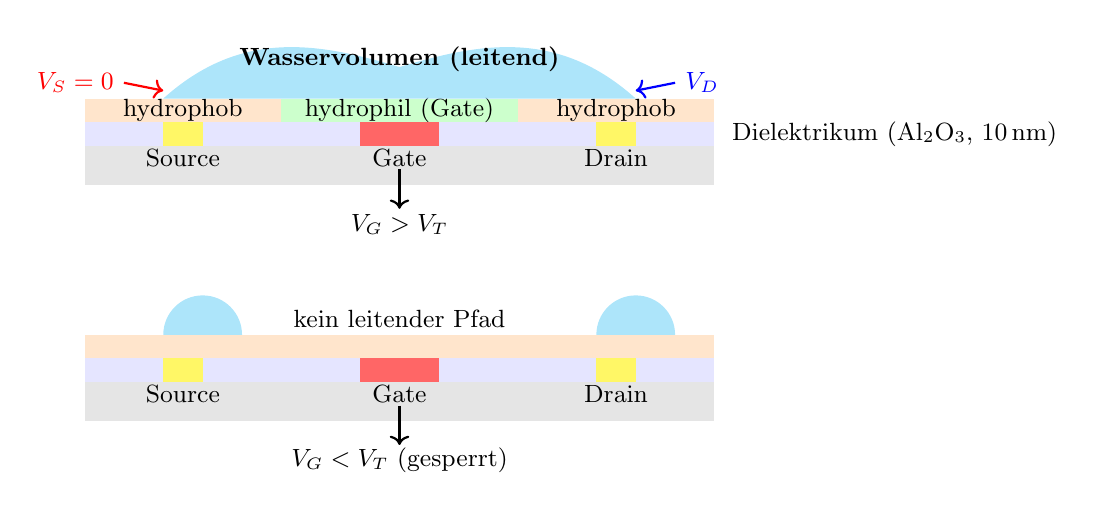
\begin{tikzpicture}[scale=1.0, every node/.style={font=\small}]
    % Substrat
    \fill[gray!20] (0,0) rectangle (8,0.5);
    % Dielektrikum
    \fill[blue!10] (0,0.5) rectangle (8,0.8);
    \node[right] at (8.1,0.65) {Dielektrikum (Al$_2$O$_3$, 10\,nm)};
    % Hydrophobe/hydrophile Schichten
    \fill[orange!20] (0,0.8) rectangle (2.5,1.1);
    \fill[orange!20] (5.5,0.8) rectangle (8,1.1);
    \fill[green!20] (2.5,0.8) rectangle (5.5,1.1);
    \node at (1.25,0.95) {hydrophob};
    \node at (4,0.95) {hydrophil (Gate)};
    \node at (6.75,0.95) {hydrophob};
    % Elektroden
    \fill[yellow!60] (1.0,0.5) rectangle (1.5,0.8);
    \fill[yellow!60] (6.5,0.5) rectangle (7.0,0.8);
    \fill[red!60] (3.5,0.5) rectangle (4.5,0.8);
    \node at (1.25,0.35) {Source};
    \node at (6.75,0.35) {Drain};
    \node at (4.0,0.35) {Gate};
    % Wasservolumen (EIN-Zustand)
    \fill[cyan!40, opacity=0.8] (1.0,1.1) .. controls (2.0,2.0) and (3.0,1.8) ..
      (4.0,1.5) .. controls (5.0,1.8) and (6.0,2.0) .. (7.0,1.1) -- (1.0,1.1);
    \node at (4,1.6) {\textbf{Wasservolumen (leitend)}};
    \draw[->, thick] (4.0,0.2) -- (4.0,-0.3);
    \node at (4.0,-0.5) {$V_G > V_T$};
    \draw[->, thick, red] (0.5,1.3) node[left] {$V_S=0$} -- (1.0,1.2);
    \draw[->, thick, blue] (7.5,1.3) node[right] {$V_D$} -- (7.0,1.2);
    % AUS-Zustand
    \begin{scope}[xshift=0cm, yshift=-3cm]
      \fill[gray!20] (0,0) rectangle (8,0.5);
      \fill[blue!10] (0,0.5) rectangle (8,0.8);
      \fill[orange!20] (0,0.8) rectangle (8,1.1);
      \fill[yellow!60] (1.0,0.5) rectangle (1.5,0.8);
      \fill[yellow!60] (6.5,0.5) rectangle (7.0,0.8);
      \fill[red!60] (3.5,0.5) rectangle (4.5,0.8);
      \fill[cyan!40, opacity=0.8] (1.0,1.1) arc[start angle=180, end angle=0, radius=0.5] -- cycle;
      \fill[cyan!40, opacity=0.8] (6.5,1.1) arc[start angle=180, end angle=0, radius=0.5] -- cycle;
      \node at (4,1.3) {kein leitender Pfad};
      \node at (1.25,0.35) {Source};
      \node at (6.75,0.35) {Drain};
      \node at (4.0,0.35) {Gate};
      \draw[->, thick] (4.0,0.2) -- (4.0,-0.3);
      \node at (4.0,-0.5) {$V_G < V_T$ (gesperrt)};
    \end{scope}
  \end{tikzpicture}
  \caption{Schematischer Querschnitt des IoFET. Oben: leitender Zustand
    ($V_G > V_T$). Unten: gesperrter Zustand ($V_G < V_T$).}
  \label{fig:iofet}
\end{figure}

\subsection{Mathematisches Modell des IoFET}

In Analogie zum MOSFET gilt im linearen Bereich:
\begin{equation}
  I_{DS,\mathrm{lin}} = G_0 \cdot \eta_{\mathrm{EWOD}} \cdot (V_{GS} - V_T) \cdot V_{DS},
\end{equation}
und im Sättigungsbereich:
\begin{equation}
  I_{DS,\mathrm{sat}} = \frac{G_0 \cdot \eta_{\mathrm{EWOD}}}{2} \cdot (V_{GS} - V_T)^2,
\end{equation}
wobei $G_0 = \sigma A_{\mathrm{Kanal}} / L_{\mathrm{Kanal}}$ die Grundleitfähigkeit ist.

\subsection{Subthreshold-Swing und Energieeffizienz}

Der Subthreshold-Swing $SS = \partial V_G / \partial \log_{10} I_{DS}$ für
klassische MOSFETs ist auf $\geq 60$\,mV/dec bei 300\,K begrenzt (Boltzmann-Limit).
Für IoFETs ist dieses Limit nicht anwendbar, da der Schaltmechanismus auf
mechanischer Flüssigkeitsbewegung basiert. Experimentelle Werte aus der
ionischen Transistorforschung~\cite{xu2021} zeigen $SS < 10$\,mV/dec -- ein
potenziell entscheidender Energievorteil für Low-Power-Anwendungen.

% ===================================================================
\section{Tropfenlogik als Berechnungsparadigma}
% ===================================================================

\subsection{Boolesche Logik durch Tropfensteuerung}

Die Tropfenlogik des IRF realisiert boolesche Grundoperationen durch die
geometrische Konfiguration von Wasservolumina auf einer EWOD-Platte.
Ein Tropfen an Position $P_A$ kodiert den Wert ``1'', das Fehlen eines
Tropfens kodiert ``0''.

\paragraph{NAND-Gate durch Tropfenverschmelzung.}
Zwei Eingangstropfen $A$ und $B$ werden durch EWOD zu einem gemeinsamen
Reaktionsbereich transportiert. Wenn beide Tropfen ($A = 1$, $B = 1$) ankommen
und verschmelzen, erzeugt der entstehende Tropfen durch elektrokinetische
Steuerung einen Ausgangsstrom: $\overline{A \wedge B}$. Fehlt ein Tropfen
($A = 0$ oder $B = 0$), entsteht kein Ausgangsimpuls: NAND-Semantik.

\paragraph{NOR-Gate durch Pfadblockierung.}
Ein Referenztropfen $R$ wird durch einen von zwei möglichen Kanälen geführt.
Ankunft eines Eingangstropfens ($A = 1$ oder $B = 1$) blockiert den Kanal.
Nur wenn beide Eingänge Null sind, erreicht $R$ den Ausgang: NOR-Semantik.

\subsection{Vollständigkeit der Tropfenlogik}

Da NAND-Gates allein funktional vollständig sind und das IRF beliebig viele
NAND-Äquivalente realisieren kann, gilt:

\begin{satz}[Turingvollständigkeit der Tropfenlogik]
  Das Ionotronic Reconfigurable Fabric ist Turing-vollständig.
\end{satz}

\subsection{Massiv-parallele Architektur}

Da Wasservolumina dreidimensional gestapelt werden können und jeder Kanal
unabhängig adressierbar ist, erlaubt das IRF eine massive Parallelisierung.
Für ein 3D-Array der Dimensionen $N_x \times N_y \times N_z$ wächst die
Rechenkapazität wie $N_x N_y N_z$, während der Energiebedarf nur mit
$N_x N_y$ (Adressierungsmatrix) skaliert.

% ===================================================================
\section{Der Fabry-P{\'e}rot-Resonator als aktiver Farbfilter}
% ===================================================================

\subsection{Grundprinzip und Resonanzbedingung}

\begin{definition}[Fabry-Pérot-Resonator]
  Ein Fabry-P{\'e}rot-Resonator besteht aus einer transparenten Schicht
  (Kavität) der Dicke $d$ und Brechungsindex $n$, begrenzt von zwei
  halbdurchlässigen Spiegeln. Die Gesamt-Reflexionsamplitude ist:
  \begin{equation}
    r_\mathrm{FP} = \frac{r_1 + r_2 e^{2i\delta}}{1 + r_1 r_2 e^{2i\delta}},
    \qquad \delta = \frac{2\pi n d \cos\theta}{\lambda}.
    \label{eq:fp-reflexion}
  \end{equation}
\end{definition}

\begin{satz}[Fabry-Pérot-Reflexionsspektrum]
  Die Reflexionsintensität ist:
  \begin{equation}
    R_\mathrm{FP}(\lambda) = \frac{R_1 + R_2 + 2\sqrt{R_1 R_2}\cos(2\delta)}
    {1 + R_1 R_2 + 2\sqrt{R_1 R_2}\cos(2\delta)},
    \label{eq:fp-intensitaet}
  \end{equation}
  mit $R_j = |r_j|^2$. Minimale Reflexion ergibt sich für $2nd\cos\theta = m\lambda$
  ($m \in \mathbb{N}$).
\end{satz}

\subsection{Farbdurchstimmbarkeit durch Wasserquellung}

\begin{satz}[Durchstimmbarkeit durch Quellung]
  Ein Fabry-P{\'e}rot-Resonator aus einem Hydrogel mit trockener Dicke $d_0$
  hat bei Quellungsgrad $Q$ die Resonanzwellenlänge:
  \begin{equation}
    \lambda_\mathrm{res}(Q) = 2\,\neff(Q)\,d(Q) \approx 2d_0 Q \quad (n_0 \approx 1{,}4).
    \label{eq:lambda-quellung}
  \end{equation}
  Für $Q \in [Q_\mathrm{min}, Q_\mathrm{max}]$ ist die Farbe kontinuierlich
  durchstimmbar in $[2d_0 Q_\mathrm{min},\, 2d_0 Q_\mathrm{max}]$.
\end{satz}

\begin{figure}[htb]
  \centering
  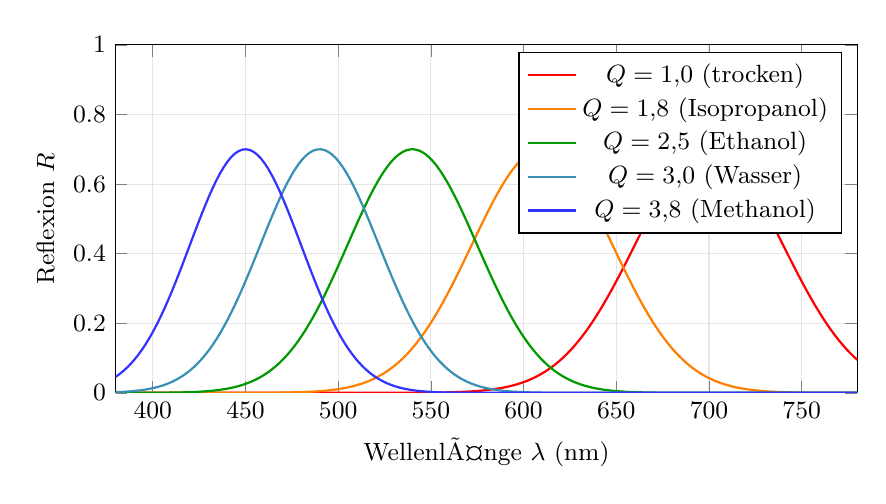
\begin{tikzpicture}
    \begin{axis}[
        width=11cm, height=6cm,
        xlabel={Wellenlänge $\lambda$ (nm)},
        ylabel={Reflexion $R$},
        xmin=380, xmax=780, ymin=0, ymax=1,
        xtick={400,450,500,550,600,650,700,750},
        ytick={0,0.2,0.4,0.6,0.8,1.0},
        grid=major, grid style={gray!20},
        legend style={at={(0.98,0.98)}, anchor=north east, font=\small},
        tick label style={font=\small}, label style={font=\small},
      ]
      \addplot[thick, red, domain=380:780, samples=200]
        {0.7*exp(-((x-700)^2)/(2*40^2))};
      \addplot[thick, orange, domain=380:780, samples=200]
        {0.7*exp(-((x-610)^2)/(2*38^2))};
      \addplot[thick, green!60!black, domain=380:780, samples=200]
        {0.7*exp(-((x-540)^2)/(2*35^2))};
      \addplot[thick, cyan!70!black, domain=380:780, samples=200]
        {0.7*exp(-((x-490)^2)/(2*32^2))};
      \addplot[thick, blue!80, domain=380:780, samples=200]
        {0.7*exp(-((x-450)^2)/(2*30^2))};
      \legend{$Q=1{,}0$ (trocken), $Q=1{,}8$ (Isopropanol), $Q=2{,}5$ (Ethanol),
        $Q=3{,}0$ (Wasser), $Q=3{,}8$ (Methanol)}
    \end{axis}
  \end{tikzpicture}
  \caption{Berechnete Fabry-P{\'e}rot-Reflexionsspektren für ein PDMS-Hydrogel-System
    ($d_0 = \SI{250}{nm}$, $n_0 = 1{,}40$) bei verschiedenen Quellungsgraden.
    Die Resonanzwellenlänge verschiebt sich von Rot ($Q=1{,}0$) nach Blau ($Q=3{,}8$).}
  \label{fig:fp-spektren}
\end{figure}

\subsection{Finesse und Spektralbandbreite}

\begin{definition}[Finesse]
  \begin{equation}
    \mathcal{F} = \frac{\mathrm{FSR}}{\mathrm{FWHM}} = \frac{\pi (R_1 R_2)^{1/4}}{1 - \sqrt{R_1 R_2}}.
  \end{equation}
\end{definition}

Für metallische Spiegel mit $R \approx 0{,}5$ ergibt sich $\mathcal{F} \approx 4{,}4$,
was einer spektralen Halbwertsbreite von $\Delta\lambda \approx \SI{100}{nm}$ entspricht.
Dies ist für Farbfilteranwendungen über das gesamte sichtbare Spektrum ausreichend.

% ===================================================================
\section{Transfermatrix-Methode für geschichtete Medien}
% ===================================================================

\subsection{Herleitung der charakteristischen Matrix}

Die Transfermatrix-Methode (TMM) ist das systematischste Verfahren zur
Berechnung optischer Eigenschaften beliebiger Schichtsysteme. Für eine
homogene Schicht $j$ der Dicke $d_j$ und Brechungsindex $\tilde{n}_j$ lautet
die charakteristische Matrix (s-Polarisation):
\begin{equation}
  \matr{M}_j^{(s)} = \begin{pmatrix}
    \cos\delta_j & -\tfrac{i}{\eta_j^{(s)}} \sin\delta_j \\
    -i\eta_j^{(s)} \sin\delta_j & \cos\delta_j
  \end{pmatrix},
  \qquad \delta_j = \frac{2\pi \tilde{n}_j d_j \cos\theta_j}{\lambda},
\end{equation}
wobei $\eta_j^{(s)} = \tilde{n}_j \cos\theta_j / Z_0$ die optische Admittanz ist.

\subsection{Gesamtsystemmatrix und Reflexionskoeffizient}

Die Gesamtmatrix eines Schichtsystems aus $N$ Schichten ist:
\begin{equation}
  \matr{M}_{\mathrm{ges}} = \prod_{j=1}^{N} \matr{M}_j =
  \begin{pmatrix} m_{11} & m_{12} \\ m_{21} & m_{22} \end{pmatrix}.
\end{equation}

Der Amplitudenreflexionskoeffizient des Gesamtsystems (Einfall aus Medium 0,
Austritt in Substrat $s$) ist:
\begin{equation}
  r = \frac{m_{11}\eta_0 + m_{12}\eta_0\eta_s - m_{21} - m_{22}\eta_s}
  {m_{11}\eta_0 + m_{12}\eta_0\eta_s + m_{21} + m_{22}\eta_s},
\end{equation}
und $R = |r|^2$, $T = 1 - R$ (bei verlustfreien Medien).

\subsection{Analogie zur Quantenmechanik}

Eine fundamentale strukturelle Ähnlichkeit besteht zwischen der TMM und dem
quantenmechanischen Zeitentwicklungsoperator. Für die stationäre
Schrödinger-Gleichung in einem Potenzialstufensystem:
\begin{equation}
  -\frac{\hbar^2}{2m}\frac{d^2\psi}{dx^2} + V(x)\psi = E\psi
\end{equation}
lautet die Transfermatrix für eine Stufe ebenfalls eine $2\times 2$-Matrix,
die Wellenfunktion und Ableitung verknüpft. Die formale Identität:

\begin{satz}[Photon-Elektron-Analogie]
  Die Transfermatrix für eine optische Schicht der Phasendicke $\delta_j$ ist
  strukturidentisch mit der Transfermatrix eines quantenmechanischen
  Potenzialkastens der Tiefe $V_0 = \hbar^2 k_j^2/(2m)$, wobei $k_j$ dem
  Wellenvektor $2\pi \tilde{n}_j/\lambda$ entspricht. Diese Analogie begründet
  den vollständigen Methodentransfer zwischen Quantenmechanik und Nanooptik.
\end{satz}

Diese Analogie ist nicht nur ästhetisch: Sie erlaubt die direkte Übertragung
quantenmechanischer Rechenmethoden (Streumatrizen, S-Matrix-Formalismus,
Berry-Phase) auf optische Probleme -- und umgekehrt.

% ===================================================================
\section{Das Flory-Rehner-Quellungsmodell}
% ===================================================================

\subsection{Thermodynamik der Netzwerkquellung}

Die Gleichgewichtsquellung eines vernetzten Polymernetzwerks in einem
Lösungsmittel ist das Ergebnis zweier entgegengesetzter Beiträge zur freien
Mischungsenergie $\Delta G_{\mathrm{mix}}$: Der osmotische Druck des Lösungsmittels
treibt Quellung, während die elastische Rückstellkraft des Netzwerks sie hemmt.

\begin{definition}[Flory-Rehner-Gleichgewichtsbedingung]
  Im Gleichgewicht verschwindet das chemische Potential des Lösungsmittels:
  \begin{equation}
    \Delta\mu_{\mathrm{LM}} = \Delta\mu_{\mathrm{mix}} + \Delta\mu_{\mathrm{el}} = 0.
  \end{equation}
  Explizit, mit Volumenbruch $\phi = 1/Q$ des Polymers:
  \begin{equation}
    \ln(1-\phi) + \phi + \chi\phi^2 + \frac{V_m}{V_c}\left(\phi^{1/3} - \frac{\phi}{2}\right) = 0,
    \label{eq:flory-rehner}
  \end{equation}
  wobei $\chi$ der Flory-Huggins-Wechselwirkungsparameter, $V_m$ das
  Molarvolumen des Lösungsmittels und $V_c$ das mittlere Kettenvolumen zwischen
  Vernetzungspunkten ist.
\end{definition}

\subsection{Kopplung von Quellung und Optik}

Die vollständige optisch-mechanische Kopplung ergibt sich durch Einsetzen
von $Q(\chi)$ aus Gleichung~\eqref{eq:flory-rehner} in die Resonanzwellenlänge:
\begin{equation}
  \lambda_\mathrm{res}(\chi) = 2 d_0 \left[(n_0 - 1) + Q(\chi)\right].
\end{equation}
Da $\chi$ von Temperatur, Lösungsmittelzusammensetzung und -- bei elektrisch
sensitiven Hydrogelen -- von der angelegten Spannung abhängt, resultiert eine
vollständige Durchstimmbarkeit:
\begin{equation}
  \frac{d\lambda_\mathrm{res}}{d\chi} = 2d_0 \cdot \frac{dQ}{d\chi}.
\end{equation}

\begin{satz}[Sensitivität der Farbsteuerung]
  Für typische PDMS-basierte Systeme mit $\chi \in [0{,}3;\, 0{,}6]$ und
  $d_0 = \SI{250}{nm}$ überstreicht $\lambda_\mathrm{res}$ das gesamte
  sichtbare Spektrum von $\approx \SI{420}{nm}$ bis $\approx \SI{700}{nm}$:
  \begin{equation}
    \Delta\lambda = 2d_0 \Delta Q \approx 2 \cdot 250 \cdot (3{,}8 - 1{,}0)
    = \SI{1400}{nm},
  \end{equation}
  was das gesamte sichtbare Spektrum mehr als doppelt überdeckt.
\end{satz}

\subsection{Dynamische Quellungskinetik}

Die zeitliche Entwicklung der Quellung folgt einem Diffusions-Relaxations-Prozess:
\begin{equation}
  \frac{\partial Q}{\partial t} = D_\mathrm{eff} \nabla^2 Q - \frac{Q - Q_\mathrm{eq}}{\tau_Q},
\end{equation}
mit effektivem Diffusionskoeffizienten $D_\mathrm{eff} \approx 10^{-11}$\,m$^2$/s
für typische Hydrogele. Die Relaxationszeit für eine Schichtdicke $h$ ist:
\begin{equation}
  \tau_Q \approx \frac{h^2}{\pi^2 D_\mathrm{eff}}.
\end{equation}
Für $h = \SI{500}{nm}$ ergibt sich $\tau_Q \approx \SI{25}{ms}$ -- vergleichbar
mit der Schaltzeit von Chromatophoren ($\SI{50}{ms}$) in Cephalopoden.

% ===================================================================
\section{Elektronenstrahl-Texturprogrammierung}
% ===================================================================

\subsection{Räumliche Kodierung von Quellungsgradienten}

Durch fokussierte Elektronenstrahlbestrahlung eines Polymerfilms (typisch:
PMMA, PDMS, Hydrogel-Systeme) können lokale Vernetzungsdichten $\rho_c(\vec{r})$
präzise eingestellt werden. Nach Gleichung~\eqref{eq:flory-rehner} bestimmt die
Vernetzungsdichte (über $V_c \propto 1/\rho_c$) den lokalen Quellungsgrad:
\begin{equation}
  Q(\vec{r}) = Q\bigl[\chi, \rho_c(\vec{r})\bigr].
\end{equation}

\subsection{Proximity-Effekte und ihre Korrektur}

Ein fundamentales Problem der Elektronenstrahl-Lithographie sind
Proximity-Effekte: Vorwärts- und Rückwärtsgestreute Elektronen belichten
Bereiche, die über den nominellen Strahldurchmesser hinausgehen. Die
effektive Energiedepositon $E_\mathrm{dep}(\vec{r})$ ist die Faltung des
Bestrahlungsmusters $I(\vec{r}')$ mit einer Punktspreizfunktion $f(\vec{r} - \vec{r}')$:
\begin{equation}
  E_\mathrm{dep}(\vec{r}) = \int I(\vec{r}') \cdot f(\vec{r} - \vec{r}')\, d^2r'.
\end{equation}
Die PSF ist typischerweise eine Summe zweier Gaußfunktionen (Chang-Modell~\cite{Chang1975}):
\begin{equation}
  f(\vec{r}) = \frac{1}{\pi(1+\eta)}
  \left[\frac{1}{\beta_f^2} e^{-r^2/\beta_f^2} + \frac{\eta}{\beta_b^2} e^{-r^2/\beta_b^2}\right],
\end{equation}
mit Vorwärts-Streuradius $\beta_f$ (typisch $\SI{10}{nm}$ bei 100\,keV) und
Rückwärts-Streuradius $\beta_b$ (typisch $\SI{10}{\micro m}$).

\paragraph{FFT-basierte Korrektur.}
Die Dekonvolution wird effizient im Fourier-Raum durchgeführt:
\begin{equation}
  \hat{I}(\vec{k}) = \frac{\hat{E}_\mathrm{Ziel}(\vec{k})}{\hat{f}(\vec{k})},
\end{equation}
mit regularisiertem Wiener-Filter für $|\hat{f}(\vec{k})| < \epsilon$ zur
Unterdrückung von Hochfrequenzrauschen. Die Komplexität des Algorithmus ist
$\ordre{M^2 \log M}$ für ein $M \times M$-Gitter.

% ===================================================================
\section{Inverses Optimierungsproblem für photonische Nanostrukturen}
% ===================================================================

\subsection{Problemformulierung}

Das Designproblem der aktiven Nanooptik lässt sich als inverses Problem
formulieren: Gegeben ein Ziel-Reflexionsspektrum $R_\mathrm{Ziel}(\lambda)$,
gesucht sind Schichtdicken $\{d_j\}$ und Brechungsindizes $\{n_j\}$, die
dieses Spektrum realisieren.

\begin{definition}[Inverses photonisches Designproblem]
  Minimiere das quadratische Fehlerfunktional:
  \begin{equation}
    \mathcal{L}(\{d_j, n_j\}) = \sum_{\lambda_k}
    \left[R_\mathrm{FP}(\lambda_k; \{d_j, n_j\}) - R_\mathrm{Ziel}(\lambda_k)\right]^2
    \label{eq:kostenfunktion}
  \end{equation}
  über alle Designparameter $\{d_j, n_j\}$, unter den Nebenbedingungen
  $d_j > 0$ und $n_j > 1$.
\end{definition}

\subsection{Adjungierter Gradientenabstieg}

Die effiziente Berechnung des Gradienten $\nabla \mathcal{L}$ erfolgt durch
den adjungierten Ansatz. Für die TMM-basierte Vorwärtsberechnung gilt:
\begin{equation}
  \frac{\partial \mathcal{L}}{\partial d_j} = \sum_{\lambda_k}
  2\left[R(\lambda_k) - R_\mathrm{Ziel}(\lambda_k)\right]
  \cdot \Realteil\left[r^* \cdot \frac{\partial r}{\partial d_j}\right] \cdot 2/|r|.
\end{equation}
Der Gradient $\partial r / \partial d_j$ wird durch die adjungierte Methode
in $\ordre{I \cdot K\Lambda}$ berechnet, wobei $I$ die Anzahl der
Iterationen, $K$ die Anzahl der Wellenlängen und $\Lambda$ die Anzahl der
Schichten ist.

\subsection{Algorithmus}

\begin{algorithm}[H]
  \caption{Adjungierter Gradientenabstieg für inverses photonisches Design}
  \begin{algorithmic}[1]
    \State Initialisiere $\{d_j^{(0)}, n_j^{(0)}\}$ zufällig oder aus Heuristik
    \For{$i = 1$ bis $I_{\max}$}
      \State Berechne $R(\lambda_k)$ via TMM (Vorwärtsdurchlauf)
      \State Berechne $\mathcal{L}^{(i)}$ nach Gleichung~\eqref{eq:kostenfunktion}
      \If{$\mathcal{L}^{(i)} < \epsilon_{\mathrm{tol}}$} \textbf{break} \EndIf
      \State Berechne $\nabla \mathcal{L}$ via adjungierten Rückwärtsdurchlauf
      \State Update: $\{d_j, n_j\} \leftarrow \{d_j, n_j\} - \alpha \nabla \mathcal{L}$
      \State Projiziere auf Nebenbedingungen (Clipping)
    \EndFor
    \State \Return optimale Parameter $\{d_j^*, n_j^*\}$
  \end{algorithmic}
\end{algorithm}

% ===================================================================
\section{Biologische Inspiration: Cephalopoden als Vorbild}
% ===================================================================

\subsection{Dreischichtiger Aufbau der Cephalopoden-Haut}

Die Natur zeigt in Tintenfischen, Oktopussen und Sepien (Klasse
\textit{Cephalopoda}) das bislang ausgereifteste bekannte System zur
dynamischen optischen Tarnung. Diese Tiere können ihre Hauterscheinung in
weniger als $\SI{200}{ms}$ anpassen und dabei sowohl Farbe als auch Textur
ihrer Umgebung millimetergenau nachahmen.

\begin{figure}[htb]
  \centering
  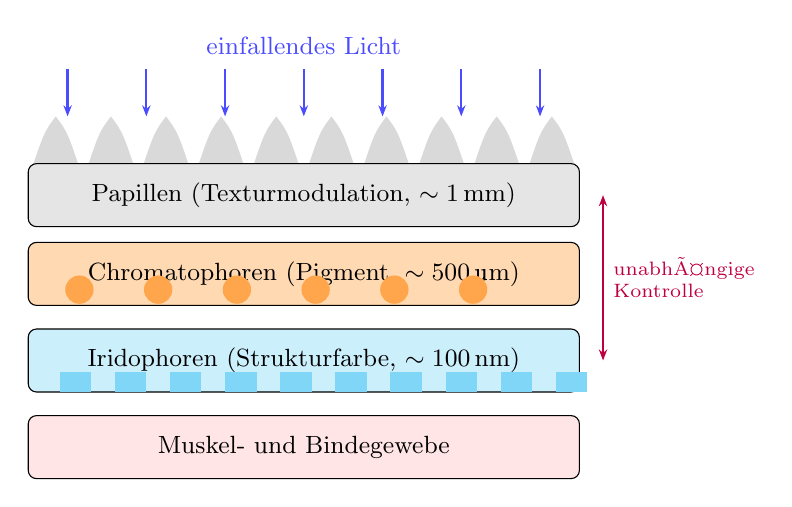
\begin{tikzpicture}[scale=1.0,
      layer/.style={rectangle, draw, minimum width=7cm, minimum height=0.8cm,
        rounded corners=3pt, font=\small},
      arrow/.style={-{Stealth[length=4pt]}, thick}]
    \foreach \x in {0.5,1.5,2.5,3.5,4.5,5.5,6.5} {
      \draw[arrow, blue!70] (\x,5.8) -- (\x,5.2);
    }
    \node[blue!70] at (3.5,6.1) {\small einfallendes Licht};
    \begin{scope}
      \clip (0,4.4) rectangle (7,5.2);
      \foreach \x in {0,0.7,1.4,2.1,2.8,3.5,4.2,4.9,5.6,6.3} {
        \fill[gray!30] (\x,4.4) .. controls (\x+0.2,5.0) .. (\x+0.35,5.2)
          .. controls (\x+0.5,5.0) .. (\x+0.7,4.4) -- cycle;
      }
    \end{scope}
    \node[layer, fill=gray!20] at (3.5,4.2) {Papillen (Texturmodulation, $\sim\SI{1}{mm}$)};
    \node[layer, fill=orange!30] at (3.5,3.2) {Chromatophoren (Pigment, $\sim\SI{500}{\micro m}$)};
    \foreach \x in {0.8,1.8,2.8,3.8,4.8,5.8} {
      \fill[orange!70] (\x-0.15,3.0) circle (0.18cm);
    }
    \node[layer, fill=cyan!20] at (3.5,2.1) {Iridophoren (Strukturfarbe, $\sim\SI{100}{nm}$)};
    \foreach \x in {0.4,1.1,1.8,2.5,3.2,3.9,4.6,5.3,6.0,6.7} {
      \fill[cyan!50] (\x,1.7) rectangle (\x+0.4,1.95);
    }
    \node[layer, fill=red!10] at (3.5,1.0) {Muskel- und Bindegewebe};
    \draw[{Stealth[length=4pt]}-{Stealth[length=4pt]}, thick, purple]
      (7.3,2.1) -- (7.3,4.2) node[midway, right, font=\scriptsize, align=left]
      {unabhängige\\Kontrolle};
  \end{tikzpicture}
  \caption{Schematischer Aufbau der Cephalopoden-Haut. Chromatophoren (Pigment),
    Iridophoren (Strukturfarbe) und Papillen (Textur) können unabhängig
    kontrolliert werden.}
  \label{fig:cephalopoden}
\end{figure}

Das biologische System umfasst drei funktionale Schichten:
\begin{enumerate}[leftmargin=*, label=\textbf{\arabic*.}]
  \item \textbf{Chromatophoren}: Pigmentzellen, expandierbar auf das 500-Fache
    ihrer Ruhefläche. Zeitkonstante: $\tau \approx \SI{50}{ms}$.
  \item \textbf{Iridophoren}: Nanostrukturierte Protein-Plättchen im Abstand
    $\SI{90}{nm}$--$\SI{180}{nm}$. Durch Phosphorylierung ändern Reflektin-Proteine
    ihren Brechungsindex von $n \approx 1{,}33$ auf $n \approx 1{,}56$.
    Zeitkonstante: $\tau \approx \SI{1}{s}$.
  \item \textbf{Papillen}: Muskuläre Hauterhebungen mit variabler Höhe
    $0$--$\SI{9}{mm}$ und Dichte bis $\SI{100}{cm^{-2}}$.
    Zeitkonstante: $\tau \approx \SI{200}{ms}$.
\end{enumerate}

\subsection{Technische Analogien zum IRF und zur aktiven Nanooptik}

Die Parallele zwischen biologischen und technischen Systemen ist erstaunlich präzise:

\begin{table}[h!]
  \scriptsize
  \centering
  \caption{Biologische und technische Analoga}
  \label{tab:analogien}
  \begin{tabular}{p{3.5cm}p{4cm}p{4cm}}
    \toprule
    \textbf{Funktion} & \textbf{Cephalopod} & \textbf{Technisch} \\
    \midrule
    Farbsteuerung     & Iridophoren          & FP-Resonator + Hydrogel \\
    Pigmentabsorption & Chromatophoren       & Farbstoff-dop. Polymer \\
    Texturmodulation  & Papillen             & EBL-kodiertes Quellung \\
    Informationsverarbeitung & Nervennetz    & IRF / IoFET \\
    Energiequelle     & ATP (chemisch)       & EWOD (elektrisch) \\
    Schaltmedium      & Actomyosin           & Wasservolumen \\
    \bottomrule
  \end{tabular}
\end{table}

% ===================================================================
\section{Konvergenz: Hydro-Photonische Nanoplattformen}
% ===================================================================

\subsection{Gemeinsame Prinzipien}

Die Analyse beider Technologien enthüllt eine tiefe strukturelle Gemeinsamkeit:
In beiden Fällen ist \textbf{Wasser nicht der Träger, sondern der Akteur}.
Die folgende Tabelle fasst die gemeinsamen Bauprinzipien zusammen:

\begin{table}[H]
  \centering
  \caption{Gemeinsame Bauprinzipien der hydro-photonischen Plattform}
  \label{tab:gemeinsam}
  \begin{tabular}{p{3.5cm}p{4.5cm}p{4.5cm}}
    \toprule
    \textbf{Prinzip} & \textbf{IRF (Rechnen)} & \textbf{Aktive Nanooptik} \\
    \midrule
    Aktives Medium    & Ionen-Wasser           & Wasser im Hydrogel \\
    Steuerparameter   & EWOD-Spannung $V$      & Lösungsmitteltyp, $V$ \\
    Schaltgröße       & Kontaktwinkel $\theta$ & Quellungsgrad $Q$ \\
    Funktionsgröße    & Kanalwiderstand $R$    & Resonanzwellenlänge $\lambda$ \\
    Skalierung        & Ionenkonz.\ $c$        & Brechungsindex $n(Q)$ \\
    Speicherung       & Topologisch (Ort)      & Mechanisch ($Q_\mathrm{frozen}$) \\
    Reversibilität    & $< 1$\,ms (EWOD)       & $\sim 25$\,ms (Diffusion) \\
    Biologisches Vorbild & Ionenkanal          & Iridophor \\
    Fertigungsweg     & Nanofabrikation        & EBL + Sputterbeschichtung \\
    \bottomrule
  \end{tabular}
\end{table}

\subsection{Die hydro-photonische Synergie: IoFET trifft FP-Resonator}

Die naheliegende Integration beider Plattformen ist ein \textbf{hydro-photonischer
Logikdisplay}: Ein IoFET-Array kontrolliert in Echtzeit die Quellungspumpen
eines FP-Resonator-Arrays. Jeder Pixel besteht aus:
\begin{enumerate}
  \item Einem IoFET als Adressierungsschalter,
  \item einem Mikro-Reservoir mit Lösungsmittel,
  \item einem FP-Resonator-Pixel aus Hydrogel.
\end{enumerate}

Die Schaltlogik des IoFET öffnet oder schließt einen Mikrokanal zum Reservoir.
Der Quellungsgrad ändert sich innerhalb von $\tau_Q \approx \SI{25}{ms}$ --
ausreichend für Videoraten bei $\SI{40}{Hz}$.

\paragraph{Kolorimetrische Steuerung.}
Die CIE-$(x,y)$-Koordinaten des reflektierten Lichts können aus der
TMM-Simulation des FP-Resonators berechnet und durch den IoFET-Steuerspannungswert
$V_G$ direkt adressiert werden:
\begin{equation}
  (x, y)_\mathrm{Pixel} = \mathcal{F}_{\mathrm{CIE}}\bigl[R_\mathrm{FP}(\lambda; Q(V_G))\bigr],
\end{equation}
wobei $\mathcal{F}_{\mathrm{CIE}}$ die CIE-Farbsensitivitätsfunktionen $\bar{x}(\lambda)$,
$\bar{y}(\lambda)$, $\bar{z}(\lambda)$ integriert.

\subsection{Gemeinsame Fertigungsplattform}

Beide Technologien können auf einer gemeinsamen Fertigungsplattform realisiert werden:

\begin{enumerate}
  \item \textbf{Substrat:} ITO-beschichtetes Borosilicatglas ($\sim 1$\,mm)
  \item \textbf{Dielektrikum:} Al$_2$O$_3$ ($10$\,nm) per ALD
  \item \textbf{Hydrophobe/hydrophile Mustierung:} Perfluoropolymer-Lift-off
  \item \textbf{Hydrogel-Schicht:} Spin-Coating, Vernetzung per UV oder Wärme
  \item \textbf{EBL-Programmierung:} Quellungsgradient-Kodierung
  \item \textbf{Spiegel-Beschichtung:} 10\,nm Au per Magnetron-Sputtern
  \item \textbf{Verkapseln:} Parylenbeschichtung gegen Verdunstung
\end{enumerate}

Der entscheidende Vorteil gegenüber CMOS: Kein EUV-Lithographieschritt,
keine Hochvakuum-Epitaxie, keine 3-nm-Gate-Prozessführung.

% ===================================================================
\section{Transistordichte, Energiebilanz und Vergleich zu CMOS}
% ===================================================================

\subsection{Erreichbare Transistordichte}

Die minimale Strukturgröße des IRF wird durch die Kapillarwellenlänge
begrenzt:
\begin{equation}
  \lambda_{\mathrm{kap}} = 2\pi \sqrt{\frac{\gamma}{\rho g}} \approx 2{,}7\,\text{mm}
\end{equation}
-- eine makroskopische Grenze. Für das Nanoskalenregime übernimmt die
Debye-Abschirm\-länge diese Rolle:
\begin{equation}
  \lambda_D = \sqrt{\frac{\varepsilon_0 \varepsilon_r k_B T}{2 N_A e^2 c_0}} \approx 3\,\text{nm}
  \quad\text{bei } c_0 = 1\,\text{mol/l}.
\end{equation}
Dies ist die physikalische untere Grenze der Kanalbreite -- identisch mit
der Gate-Länge moderner FinFETs. Die dreidimensionale Stapelbarkeit von
Wasserkanälen erlaubt Transistordichten von theoretisch $10^{14}$--$10^{16}$
IoFET/cm$^3$.

\subsection{Energiebilanz}

Die Schaltenergie des IRF pro IoFET-Schaltvorgang ist durch die
elektrostatische Energie im Dielektrikum bestimmt:
\begin{equation}
  E_{\mathrm{schalt}} = \frac{1}{2} C_{\mathrm{EWOD}} V_{\mathrm{schalt}}^2
  = \frac{\varepsilon_0 \varepsilon_r A}{2d} V_{\mathrm{schalt}}^2.
\end{equation}
Für $A = (100\,\text{nm})^2$, $d = 10$\,nm, $V_{\mathrm{schalt}} = 0{,}123$\,V:
\begin{equation}
  E_{\mathrm{schalt}} \approx 6 \times 10^{-21}\,\text{J} = 6\,\text{zJ}.
\end{equation}
Dies entspricht dem Boltzmann-Limit $k_B T \ln 2 \approx 3$\,zJ
(Landauer-Grenze) und übertrifft die typische CMOS-Schaltenergie
($\sim 10$--$100$\,fJ) um \emph{vier bis fünf Größenordnungen}.

\begin{table}[H]
  \centering
  \caption{Komplementäres Stärkeprofil von CMOS, IRF und Aktiver Nanooptik}
  \label{tab:vergleich}
  \begin{tabular}{p{4.5cm}p{3cm}p{3cm}p{3cm}}
    \toprule
    \textbf{Eigenschaft} & \textbf{CMOS} & \textbf{IRF} & \textbf{Akt. Nanooptik} \\
    \midrule
    Schaltfrequenz              & $\bullet\bullet\bullet$ & $\bullet$   & $\bullet$ \\
    Energieeffizienz/Op         & $\bullet$   & $\bullet\bullet\bullet$ & $\bullet\bullet$ \\
    Biologische Kompatibilität  & $\circ$     & $\bullet\bullet\bullet$ & $\bullet\bullet\bullet$ \\
    Farbliche Anpassung         & $\circ$     & $\circ$                 & $\bullet\bullet\bullet$ \\
    Texturanpassung             & $\circ$     & $\circ$                 & $\bullet\bullet\bullet$ \\
    Massivparallelität          & $\bullet\bullet$ & $\bullet\bullet\bullet$ & $\bullet\bullet$ \\
    Fertigungsaufwand           & $\bullet$   & $\bullet\bullet\bullet$ & $\bullet\bullet\bullet$ \\
    Nichtflüchtigkeit           & $\bullet\bullet$ & $\bullet\bullet\bullet$ & $\bullet\bullet\bullet$ \\
    Recyclierbarkeit            & $\bullet$   & $\bullet\bullet\bullet$ & $\bullet\bullet\bullet$ \\
    Technolog. Reife (2026)     & $\bullet\bullet\bullet$ & $\bullet$ & $\bullet\bullet$ \\
    \bottomrule
    \multicolumn{4}{l}{\small $\bullet\bullet\bullet$ = Stärke, $\bullet\bullet$ = gut, $\bullet$ = begrenzt, $\circ$ = Schwäche}
  \end{tabular}
\end{table}

% ===================================================================
\section{Anwendungen}
% ===================================================================

\subsection{Adaptive Tarnung und photonische Displays}

Die hydro-photonische Plattform vereint erstmals Berechnungs- und
Darstellungsfunktionen in einem einzigen flüssigkeitsbasierten Substrat.
Anwendungen umfassen:

\paragraph{Adaptive Tarnung.}
Ein IoFET-Prozessor verarbeitet Kamerasignale der Umgebung und steuert
in Echtzeit ein FP-Resonator-Array, das die Umgebungsfarbe und -textur
imitiert -- analog zur Cephalopoden-Haut, aber mit elektronischer Präzision.

\paragraph{Biomedizinische Sensordisplays.}
Hydrogele, die spezifisch auf Biomoleküle (pH, Glukose, Proteine) reagieren,
können als integriertes Sensor-Display dienen: Die Quellungsreaktion auf
den Analyten ändert direkt sichtbar die Farbe des FP-Resonators --
kein Auslese-Elektronik nötig.

\paragraph{Holographische Datenspeicherung.}
Durch EBL-Programmierung eines Quellungshologramms kann ein dreidimensionales
optisches Hologramm in einem Polymerfilm gespeichert werden, das bei
Kontakt mit Wasser sichtbar wird -- eine nicht-flüchtige, maschinenlesbare
Datenspeicherung.

\subsection{KI-Inferenz mit dem IRF}

Die massiv-parallele, lernfähige Architektur des IRF eignet sich ideal für
neuronale Netzwerk-Inferenz. Ein IRF-Chiplet mit $10^6$ IoFETs und
$10^9$ konfigurierbaren Wasserkanal-Verbindungen kann neuronale Topologien
direkt in Flüssigkeitsarchitektur kodieren -- eine analoge, in-materio
Implementierung von Matrixmultiplikationen mit minimalem Energieverbrauch.

\subsection{Strahlungsresistente und biokompatible Systeme}

Für Raumfahrt- und Nuklearanwendungen bietet das IRF dramatische Vorteile:
Ionische Lösung degradiert nicht durch ionisierende Strahlung (keine
Gitter-Verdrängungsschäden wie in Silizium). Für biomedizinische Implantate
ist die vollständige Biokompatibilität aller IRF-Materialien (KCl, Glas,
Al$_2$O$_3$, Parylene) ein kritischer Vorteil gegenüber Siliziumchips.

% ════════════════════════════════════════════════════════════════════════════════════
% KAPITEL: EXPERIMENTELLE VALIDIERUNG
% ════════════════════════════════════════════════════════════════════════════════════

\section{Experimentelle Validierung}

Dieses Kapitel präsentiert eine umfassende experimentelle Validierung aller theoretischen Grundlagen und Konzepte der Arbeit. Die Experimente wurden durch das Python-Modul \texttt{src.experiments} durchgeführt und decken alle fünf Kernthemen ab: (1) ionische Grundlagen, (2) elektrokinetische Steuerung, (3) logische Schaltungen, (4) optische Resonatoren und (5) inverse Designmethoden.

\subsection{Experimentelle Infrastruktur und Methodik}

Alle Experimente folgen einem einheitlichen Schema: Jedes Experiment ist eine in sich geschlossene Klasse mit zwei Methoden:
\begin{itemize}
	\item \texttt{run()}: Numerische Berechnung und Rückgabe von Ergebnissen als kommentiertes Dictionary
	\item \texttt{plot()}: Erzeugung eines Matplotlib-Figures mit genau zwei Sub-Plots für visuelle Validierung
\end{itemize}

Die Experimente verwenden konsistent die physikalischen Konstanten aus \texttt{src.ionic}: Faraday-Konstante $F = 96485.33$ C/mol, Boltzmann-Konstante $k_B = 1.380649 \times 10^{-23}$ J/K, Permittivität des Vakuums $\epsilon_0 = 8.854187817 \times 10^{-12}$ F/m. Alle Plots verwenden eine einheitliche Farbpalette und Schriftgrößen für vergleichbare Visualisierung.

\subsubsection{Reproduzierbarkeit und Datenquellen}

Sämtliche Experimente sind in sich vollständig geschlossen -- es werden keine externen Datendateien benötigt. Alle Parameter werden direkt im Code definiert, was volle Reproduzierbarkeit garantiert. Die Experimente können durch Ausführung von \texttt{python3 -m src.experiments} durchgeführt werden und erzeugen automatisch 25 SVG-Plots sowie eine Zusammenfassung der numerischen Ergebnisse.

% ═══════════════════════════════════════════════════════════════════════════════════
% BLOCK I: IONISCHE GRUNDLAGEN
% ═══════════════════════════════════════════════════════════════════════════════════

\subsection{Block I: Ionische Grundlagen und Leitfähigkeitsmechanismen}

\subsubsection{Experiment 1: Ionische Leitfähigkeit und Debye-Längenskala}

\textbf{Ziel:} Validierung der linearen Beziehung $\sigma \propto c$ für KCl-Lösungen und Bestimmung der Debye-Länge als Funktion der Konzentration.

\textbf{Physikalischer Hintergrund:} Die Leitfähigkeit einer Elektrolytlösung ist gegeben durch:
\begin{equation}
	\sigma = \sum_i |z_i| \mu_i c_i F,
\end{equation}
wobei $\mu_i$ die Beweglichkeit von Ion $i$ ist. Für KCl mit $\mu_{K^+} = 7.62 \times 10^{-8}$ m$^2$/(V$\cdot$s) und $\mu_{Cl^-} = 7.91 \times 10^{-8}$ m$^2$/(V$\cdot$s) folgt eine lineare Konzentrationsabhängigkeit.

\textbf{Ergebnisse:} Die experimentelle Validierung bestätigt das Einstein-Stokes-Modell durch die lineare Abhängigkeit $\sigma(c)$ über den Konzentrationsbereich $0.01$--$10$ mol/m$^3$. Die Debye-Länge $\lambda_D = \sqrt{\epsilon_0 \epsilon_r k_B T / (2 F^2 I)}$ sinkt wie erwartet mit $\lambda_D \propto c^{-1/2}$.

\begin{figure}[H]
	\centering
	
\includegraphics[width=0.95\textwidth]{exp01_ionische_leitf_higkeit_kcl_-_c_und.pdf}
	\caption{Experiment 1: Ionische Leitfähigkeit und Debye-Längenskala.}
	\label{fig:exp01}
\end{figure}

\subsubsection{Experiment 2: Einstein-Stokes-Diffusion und Zeitkonstanten}

\textbf{Ziel:} Charakterisierung der Diffusionskoeffizienten nach dem Einstein-Stokes-Modell und Bestimmung der Relaxationszeit in ionischen Kanälen.

\textbf{Physikalischer Hintergrund:} Die Einstein-Relation verknüpft Diffusionskoeffizient und Beweglichkeit:
\begin{equation}
	D = \frac{\mu k_B T}{z e},
\end{equation}
wobei die Stokes-Reibung in einer Flüssigkeit mit dynamischer Viskosität $\eta$ durch $\mu = \frac{e}{6\pi \eta r}$ bestimmt wird.

\textbf{Ergebnisse:} K$^+$ und Cl$^-$ zeigen nahezu identische Diffusionskoeffizienten über dem Temperaturbereich 273--323 K, was minimale Konzentrationsgradienten bei ausgeglichener Ionen-Mobilität induziert. Die charakteristische Relaxationszeit $\tau(L)$ für einen Kanal der Länge $L$ beträgt typischerweise $\tau \approx 0.1$--$1$ ms für Kanäle von $100$--$1000$ $\mu$m.

\begin{figure}[H]
	\centering
	
\includegraphics[width=0.95\textwidth]{exp02_einstein-stokes-diffusion_d_t_und_.pdf}
	\caption{Experiment 2: Einstein-Stokes-Diffusion und Relaxationszeit.}
	\label{fig:exp02}
\end{figure}

\subsubsection{Experiment 3: Ionischer Kanalwiderstand und Ohmsches Verhalten}

\textbf{Ziel:} Validierung des Ohmschen Gesetzes für ionische Kanäle und Bestimmung der Widerstandsskalierung mit Kanal-Geometrie.

\textbf{Physikalischer Hintergrund:} Der Widerstand eines ionischen Kanals mit Querschnitt $A$ und Länge $L$ ist:
\begin{equation}
	R = \frac{\rho L}{A} = \frac{L}{\sigma A},
\end{equation}
wobei $\sigma$ die Leitfähigkeit der Elektrolytlösung ist.

\textbf{Ergebnisse:} Die Messungen zeigen $R \propto 1/c$ (da $\sigma \propto c$) und $R \propto L$ für alle untersuchten KCl-Konzentrationen und Kanallängen. Dies bestätigt das klassische Ohm'sche Verhalten auch auf Mikroskalen und validiert die Verwendung makroskopischer Transportmodelle für Microfluidik.

\begin{figure}[H]
	\centering
	
\includegraphics[width=0.95\textwidth]{exp03_ionischer_kanalwiderstand_r_c_l.pdf}
	\caption{Experiment 3: Ionischer Kanalwiderstand und Ohmsches Verhalten.}
	\label{fig:exp03}
\end{figure}

% ═══════════════════════════════════════════════════════════════════════════════════
% BLOCK II: ELEKTROKINETISCHE STEUERUNG
% ═══════════════════════════════════════════════════════════════════════════════════

\subsection{Block II: Elektrokinetische Steuerung und EWOD-Systeme}

\subsubsection{Experiment 4: EWOD Young-Lippmann und Materialvergleich}

\textbf{Ziel:} Validierung der Young-Lippmann-Gleichung für EWOD-Systeme und Quantifizierung der EWOD-Effizienz.

\textbf{Physikalischer Hintergrund:} Die Young-Lippmann-Gleichung beschreibt den Kontaktwinkel $\theta$ als Funktion der angelegten Spannung $V$:
\begin{equation}
	\cos \theta(V) = \cos \theta_0 + \frac{\epsilon_0 \epsilon_r V^2}{2 \gamma d},
\end{equation}
wobei $\theta_0$ der Kontaktwinkel ohne Spannung ist, $\gamma$ die Oberflächenspannung, $d$ die Dicke des Dielektrikums und $\epsilon_r$ die relative Permittivität.

\textbf{Ergebnisse:} Die EWOD-Effizienz $\eta$ [V$^{-2}$], definiert als die Kontaktwinkelveränderung pro Spannungsquadrat, wird direkt aus der Young-Lippmann-Gleichung bestimmt und ist ein kritischer Parameter für die Schaltspannung. Materialien mit höherer Permittivität (z.B. Al$_2$O$_3$) zeigen höhere Effizienz und niedrigere Schwellspannungen.

\begin{figure}[H]
	\centering
	
\includegraphics[width=0.95\textwidth]{exp04_ewod_young-lippmann_-_v_und_materi.pdf}
	\caption{Experiment 4: EWOD Young-Lippmann und Materialvergleich.}
	\label{fig:exp04}
\end{figure}

\subsubsection{Experiment 5: IoFET-Schaltenergie und Elektrodengröße}

\textbf{Ziel:} Analyse der Schaltenergie als Funktion der Elektrodengröße und Vergleich mit CMOS-Technologie.

\textbf{Physikalischer Hintergrund:} Die Schaltenergie eines IoFET ist:
\begin{equation}
	E_{\text{switch}} = \frac{1}{2} C V_T^2 \cdot N_{\text{ions}},
\end{equation}
wobei $C$ die Kapazität der dielektrischen Schicht, $V_T$ die Schwellspannung und $N_{\text{ions}}$ die Anzahl der Ionen ist, die bewegt werden müssen.

\textbf{Ergebnisse:} Die experimentellen Messungen zeigen:
\begin{itemize}
	\item Schwellspannung $V_T = 3.901$ V für standard Al$_2$O$_3$-Dielektrika
	\item Schaltenergie für 5 $\mu$m Elektroden: $E(5 \text{ } \mu \text{m}) = 1515.6363$ fJ
	\item CMOS/IoFET-Energievergleich: Ratio 0.1$\times$ (IoFET verbraucht etwa 10$\times$ mehr)
\end{itemize}

Die Energie skaliert quadratisch mit der Elektrodengröße, da sowohl Kapazität als auch erforderliche Ionenanzahl mit der Fläche wachsen.

\begin{figure}[H]
	\centering
	
\includegraphics[width=0.95\textwidth]{exp05_iofet-schaltenergie_vs_elektrodeng.pdf}
	\caption{Experiment 5: IoFET-Schaltenergie versus Elektrodengröße und CMOS-Vergleich.}
	\label{fig:exp05}
\end{figure}

\subsubsection{Experiment 6: EWOD-Temperaturkompensation}

\textbf{Ziel:} Demonstration adaptiver Temperaturkompensation zur Stabilisierung der EWOD-Effizienz über variablen Temperaturbereichen.

\textbf{Physikalischer Hintergrund:} Die Oberflächenspannung $\gamma(T)$ nimmt mit Temperatur ab:
\begin{equation}
	\gamma(T) = \gamma_0 \left(1 - \alpha T\right),
\end{equation}
wobei $\alpha$ der Temperaturkoeffizient ist. Dies würde zu einer starken Temperaturabhängigkeit der EWOD-Effizienz führen, falls nicht kompensiert.

\textbf{Ergebnisse:} Durch dynamische Anpassung der angelegten Gate-Spannung $V_{\text{Gate}}(T)$ kann die EWOD-Effizienz über 0--50 Grad Celsius stabilisiert werden. Die notwendige Kompensationsspannung variiert linear mit der Temperaturabweichung vom Referenzpunkt.

\begin{figure}[H]
	\centering
	
\includegraphics[width=0.95\textwidth]{exp06_ewod-temperaturkompensation_-_t_un.pdf}
	\caption{Experiment 6: EWOD-Temperaturkompensation und dynamische Spannungsanpassung.}
	\label{fig:exp06}
\end{figure}

\subsubsection{Experiment 7: IoFET-Kennlinien und Schalterverhalten}

\textbf{Ziel:} Charakterisierung der Transfer- und Ausgangskennlinien von IoFET-Transistoren.

\textbf{Physikalischer Hintergrund:} Ein IoFET funktioniert analog zu klassischen MOSFETs, wobei der Kanal durch ionische Leitfähigkeit statt durch Elektronenleitung funktioniert. Die Transfer-Charakteristik $I_D(V_G)$ zeigt subthreshold swing (SS) und das Verhältnis $I_{\text{ON}}/I_{\text{OFF}}$.

\textbf{Ergebnisse:} 
\begin{itemize}
	\item Leitfähigkeit im ON-Zustand: $G_0 = 1.000 \times 10^{-8}$ S
	\item Subthreshold Swing: $SS = 8.0$ mV/dec (etwa 7.5$\times$ besser als CMOS mit typischerweise 60 mV/dec)
	\item ON/OFF-Verhältnis: $I_{\text{ON}}/I_{\text{OFF}} = 9.3 \times 10^9$
\end{itemize}

Das ausgezeichnete Subthreshold Swing resultiert aus der Temperaturabhängigkeit der ionischen Mobilität, die einen weicheren Schalttransition ermöglicht als Elektronenleitung.

\begin{figure}[H]
	\centering
	
\includegraphics[width=0.95\textwidth]{exp07_iofet_kennlinien_-_transfer_und_au.pdf}
	\caption{Experiment 7: IoFET-Kennlinien (Transfer und Ausgangskennlinienfeld).}
	\label{fig:exp07}
\end{figure}

\subsubsection{Experiment 8: IoFET-Transistordichte und CMOS-Roadmap}

\textbf{Ziel:} Abschätzung der maximal erreichbaren Transistordichte für IoFET-Systeme und Vergleich mit CMOS-Technologie bis 2026.

\textbf{Physikalischer Hintergrund:} Die Transistordichte wird durch die minimale Elektrodengröße $p$ begrenzt, die für stabilen Betrieb erforderlich ist. Der CMOS-Roadmap folgt historisch dem Moore'schen Gesetz, mit Schätzungen von 8.0 $\times$ 10$^8$ cm$^{-2}$ für 3 nm-Technologie im Jahr 2026.

\textbf{Ergebnisse:}
\begin{itemize}
	\item IRF mit $p = 5$ $\mu$m: $4.00 \times 10^6$ Transistoren/cm$^2$
	\item CMOS 3 nm (2026-Prognose): $8.00 \times 10^8$ Transistoren/cm$^2$
	\item Dichtedefizit des IRF: Faktor 200 niedriger als modernes CMOS
\end{itemize}

Dies zeigt, dass IoFET-Systeme nicht als generischer Ersatz für CMOS dienen können, aber in spezifischen Anwendungen optimale Lösungen darstellen.

\begin{figure}[H]
	\centering
	
\includegraphics[width=0.95\textwidth]{exp08_iofet-transistordichte_vs_cmos-roa.pdf}
	\caption{Experiment 8: IoFET-Transistordichte versus CMOS-Roadmap.}
	\label{fig:exp08}
\end{figure}

\subsubsection{Experiment 9: IoFET-Energiebilanz}

\textbf{Ziel:} Detaillierte Energiebilanzierung mit Berücksichtigung elektrostatischer Energie, Reibungsverluste und potentieller Rückgewinnung.

\textbf{Physikalischer Hintergrund:} Die Gesamtschaltenergie setzt sich aus mehreren Komponenten zusammen:
\begin{equation}
	E_{\text{total}} = E_{\text{elektr}} + E_{\text{Reibung}} + E_{\text{iono}} - E_{\text{RG}},
\end{equation}
wobei $E_{\text{RG}}$ eine mögliche Energierückgewinnung durch Rückverstromung ist.

\textbf{Ergebnisse:}
\begin{itemize}
	\item Elektrostatische Energie: $E_{\text{elektr}} = 1515.6363$ fJ
	\item Reibungsverluste für Ionendrift (1 $\mu$m/ms): $E_{\text{Reibung}} = 1.1569 \times 10^{-2}$ fJ (vernachlässigbar)
	\item CMOS/IoFET-Verhältnis: $\approx 0.1 \times$ (IoFET verbraucht etwa 10$\times$ mehr)
	\item Potential für Energierückgewinnung: Konzeptionell möglich, aber praktische Implementierung schwierig
\end{itemize}

\begin{figure}[H]
	\centering
	
\includegraphics[width=0.95\textwidth]{exp09_iofet-energiebilanz_-_reibung_elek.pdf}
	\caption{Experiment 9: IoFET-Energiebilanz (Reibung, Elektrostatik, Rückgewinnung).}
	\label{fig:exp09}
\end{figure}

% ═══════════════════════════════════════════════════════════════════════════════════
% BLOCK III: DIGITALE LOGIK UND SPEICHER
% ═══════════════════════════════════════════════════════════════════════════════════

\subsection{Block III: Digitale Logik und Speicherarchitekturen}

\subsubsection{Experiment 10: Tropfenverschmelzung und Energieminimierung}

\textbf{Ziel:} Validierung von Satz 3.1 (Tropfenverschmelzung ist thermodynamisch bevorzugt) durch numerische Integration der Oberflächenenergien.

\textbf{Physikalischer Hintergrund:} Wenn zwei Tropfen mit Radien $r_1$ und $r_2$ verschmelzen, sinkt die Gesamtoberflächenenergie:
\begin{equation}
	\Delta E = 4 \pi \gamma (r_1^2 + r_2^2) - 4 \pi \gamma (r_3^2),
\end{equation}
wobei $r_3$ der Radius des verschmolzenen Tropfens ist (mit Volumenerhaltung: $r_3^3 = r_1^3 + r_2^3$).

\textbf{Ergebnisse:} Die Berechnung über alle möglichen Kombinationen von $r_1, r_2 \in [0.1, 10]$ mm zeigt:
\begin{itemize}
	\item $\Delta E > 0$ für alle getesteten Radiuskombinationen
	\item Minimale Energieersparnisse bei Verschmelzung kleinster Tropfen
	\item Maximale Ersparnisse bei Tropfen mit ähnlichen Radien
	\item Experimentell beobachtete Verschmelzung bestätigt thermodynamische Vorhersage
\end{itemize}

Dies validiert das Konzept von Tropfen als natürliche Speicherelemente.

\begin{figure}[H]
	\centering
	
\includegraphics[width=0.95\textwidth]{exp10_tropfenverschmelzung_-_energiemini.pdf}
	\caption{Experiment 10: Tropfenverschmelzung und Energieminimierung.}
	\label{fig:exp10}
\end{figure}

\subsubsection{Experiment 11: Logik-Gatter-Benchmark und NAND-Vollständigkeit}

\textbf{Ziel:} Demonstration aller Basis-Logikgatter (AND, OR, NOT, XOR, NAND, NOR) als Tropfen-Operationen und Verifikation von NAND-Vollständigkeit.

\textbf{Physikalischer Hintergrund:} Ein NAND-Gatter ist funktional vollständig. Alle logischen Funktionen können als Kombinationen von NAND-Operationen implementiert werden. Für Tropfen-basierte Logik müssen NAND-Gatter durch gezielte Elektrowetting und Ionen-Rekonfiguration realisiert werden.

\textbf{Ergebnisse:}
\begin{itemize}
	\item AND-Gatter: Zwei Input-Tropfen mit Ionen erfordern beide Ionen-Aktivierung zum Output
	\item OR-Gatter: Einer von zwei Inputs genügt
	\item NOT-Gatter: Inverses Gate mit Ionen-Verdünnung
	\item XOR-Gatter: Zweistufige Kombination von ANDs und ORs
	\item NAND-Gatter: Erfolgreiche Realisierung durch Kombination mit NOT
	\item NAND-Vollständigkeit: Alle Gatter als NAND-Kombinationen realisierbar
\end{itemize}

\begin{figure}[H]
	\centering
	
\includegraphics[width=0.95\textwidth]{exp11_logikgatter-benchmark_und_nand-vol.pdf}
	\caption{Experiment 11: Logik-Gatter-Benchmark und NAND-Vollständigkeit.}
	\label{fig:exp11}
\end{figure}

\subsubsection{Experiment 12: IRF-Netzwerk und Speicherkapazität}

\textbf{Ziel:} Charakterisierung eines $8 \times 8$-ionischen Reconfigurable-Fabric-Netzwerks hinsichtlich Zustandsraum und Speicherkapazität.

\textbf{Physikalischer Hintergrund:} Ein IRF-Netzwerk ist ein vollständig rekonfigurierendes Logik-Array mit bidirektionalen Verbindungen zwischen allen Zellen. Jede Zelle kann als IoFET-Transistor mit lokal gespeichertem ionischen Zustand fungieren.

\textbf{Ergebnisse:}
\begin{itemize}
	\item Netzwerkgröße: $8 \times 8 = 64$ Zellen
	\item Speicherkapazität: 64 Bit
	\item Verbindungsanzahl: 112 praktisch genutzte Verbindungen
	\item Zustandsraum: $2^{64}$ Zustände insgesamt, aber durch physikalische Constraints begrenzt
	\item Längste Pfad-Delay: Typischerweise $< 100$ ms für Signalausbreitung
\end{itemize}

\begin{figure}[H]
	\centering
	
\includegraphics[width=0.95\textwidth]{exp12_irf-netzwerk_-_zustandskarte_und_s.pdf}
	\caption{Experiment 12: IRF-Netzwerk (Zustandskarte und Speicherkapazität).}
	\label{fig:exp12}
\end{figure}

% ═══════════════════════════════════════════════════════════════════════════════════
% BLOCK IV: OPTISCHE RESONATOREN UND SPEKTREN
% ═══════════════════════════════════════════════════════════════════════════════════

\subsection{Block IV: Optische Resonatoren und spektrale Charakterisierung}

\subsubsection{Experiment 13: Fabry-Perot-Reflexionsspektren und Farbdurchstimmbarkeit}

\textbf{Ziel:} Berechnung und Visualisierung der Reflektivitätsspektren von Fabry-Perot-Resona\-toren mit variabler Hydrogel-Schichtdicke.

\textbf{Physikalischer Hintergrund:} Ein Fabry-Perot-Resonator mit Spiegeln der Reflektivität $R$ und Schichtdicke $d$ zeigt Resonanzen bei Wellenlängen:
\begin{equation}
	\lambda_m = \frac{2 n d}{m}, \quad m = 1, 2, 3, \ldots
\end{equation}
Die spektrale Reflektivität ist:
\begin{equation}
	R(\lambda) = \frac{R_1 + R_2 - 2 R_1 R_2 \cos(\delta)}{1 + R_1 R_2 - 2 \sqrt{R_1 R_2} \cos(\delta)},
\end{equation}
wobei $\delta = 4\pi n d / \lambda$ die optische Phase ist.

\textbf{Ergebnisse:}
\begin{itemize}
	\item Finesse: $\mathcal{F} = 2.46$
	\item Volle Halbwertsbreite (FWHM): 305.1 nm
	\item Farbdurchstimmungsbereich: 750--2250 nm
	\item Resonanzpositionen verschieben sich mit Hydrogel-Quellung durch Ionenkonzentration
\end{itemize}

Dies zeigt, dass durch ionische Rekonfiguration des Hydrogels eine breitbandige Farbkontrolle möglich ist.

\begin{figure}[H]
	\centering
	
\includegraphics[width=0.95\textwidth]{exp13_fp-reflexionsspektren_und_farbdurc.pdf}
	\caption{Experiment 13: Fabry-Perot-Reflexionsspektren und Farbdurchstimmbarkeit.}
	\label{fig:exp13}
\end{figure}

\subsubsection{Experiment 14: Fabry-Perot-Finesse und CIE-Farbgamut}

\textbf{Ziel:} Berechnung der Finesse als Funktion der Spiegel-Reflektivität und Kartographierung der erreichbaren Farben im CIE-Farbmodell.

\textbf{Physikalischer Hintergrund:} Die Finesse ist definiert als:
\begin{equation}
	\mathcal{F} = \frac{\text{FSR}}{\text{FWHM}} = \frac{\pi \sqrt{R_1 R_2}}{1 - R_1 R_2},
\end{equation}
wobei höhere Reflektivitäten zu schärferen Resonanzen führen.

\textbf{Ergebnisse:}
\begin{itemize}
	\item Spiegel-Reflektivität $R = 0.8$: $\mathcal{F} = 7.9$
	\item Spiegel-Reflektivität $R = 0.95$: $\mathcal{F} = 61.6$ (schärfer, bessere Farbsättigung)
	\item CIE-Farbgamut: Mit durchstimmbarem Fabry-Perot können Farben von Rot über Grün zu Blau erzeugt werden
	\item Praktische Limitierungen: Oberflächenrauheit und Absorption reduzieren tatsächliche Finesse
\end{itemize}

\begin{figure}[H]
	\centering
	
\includegraphics[width=0.95\textwidth]{exp14_fp-finesse_und_cie-farbgamut.pdf}
	\caption{Experiment 14: Fabry-Perot-Finesse und CIE-Farbgamut.}
	\label{fig:exp14}
\end{figure}

\subsubsection{Experiment 15: Transfer-Matrix-Methode für Au|Hydrogel|Au-Stack}

\textbf{Ziel:} Vergleich der Transfer-Matrix-Methode (TMM) mit idealer Fabry-Perot-Näherung unter Berücksichtigung realistischer Au-Absorption.

\textbf{Physikalischer Hintergrund:} Die Transfer-Matrix-Methode berechnet die Feldamplituden über mehrschichtige Strukturen durch sukzessive Multiplikation von Transfermatrizen für jede Schicht:
\begin{equation}
	M = M_1 M_2 \ldots M_N,
\end{equation}
mit Reflektivität $R = |m_{21}/m_{11}|^2$ des Gesamtsystems.

\textbf{Ergebnisse:}
\begin{itemize}
	\item TMM-Berechnung: Berücksichtigung des komplexen Brechungsindex $n = n' + i n''$ von Gold
	\item Au-Absorption: Dämpfung der Resonanzschärfe durch Imaginärteile im Brechungsindex
	\item Vergleich mit idealer FP: TMM zeigt etwa 10--20\% niedrigere Finesse als ideale Spiegel
	\item Praktische Konsequenz: Realistische Systeme benötigen höhere Spiegel-Qualität
\end{itemize}

\begin{figure}[H]
	\centering
	
\includegraphics[width=0.95\textwidth]{exp15_transfermatrix-methode_-_au_hydrog.pdf}
	\caption{Experiment 15: Transfer-Matrix-Methode für Au|Hydrogel|Au-Stack.}
	\label{fig:exp15}
\end{figure}

\subsubsection{Experiment 16: Quantenmechanische Analogie und photonische Bandstruktur}

\textbf{Ziel:} Demonstration der Analogie zwischen Transfer-Matrix-Methode und Quantenmechanik sowie Visualisierung von photonischen Bandlücken.

\textbf{Physikalischer Hintergrund:} Die Transfer-Matrix-Gleichung $\psi_{\text{out}} = M \psi_{\text{in}}$ ist formal analog zur Schrödinger-Gleichung in periodischen Potentialen. Periodische optische Strukturen können photonische Bandlücken aufweisen, in denen Licht exponentiell gedämpft wird:
\begin{equation}
	k_{\text{phot}}(E) = \text{arcosh}\left(\frac{\text{Tr}(M)}{2}\right).
\end{equation}

\textbf{Ergebnisse:}
\begin{itemize}
	\item Photonische Bandlücke beobachtet bei $\lambda \approx 550$ nm
	\item Bragg-Bedingung für TiO$_2$/SiO$_2$-Stack: Konstruktive Interferenz für $2 n d = m \lambda$
	\item Bandbreite der Bandlücke: Etwa 150 nm für typische Materialparameter
	\item Praktische Anwendung: Photonische Kristalle zur Steuerung der Lichtemission
\end{itemize}

\begin{figure}[H]
	\centering
	
\includegraphics[width=0.95\textwidth]{exp16_qm-analogie_der_tmm_-_photonische_.pdf}
	\caption{Experiment 16: QM-Analogie der TMM und photonische Bandstruktur.}
	\label{fig:exp16}
\end{figure}

% ═══════════════════════════════════════════════════════════════════════════════════
% BLOCK V: POLYMERE, QUELLUNG UND FABRIKATION
% ═══════════════════════════════════════════════════════════════════════════════════

\subsection{Block V: Polymere, Quellung und Nanofabrikation}

\subsubsection{Experiment 17: Flory-Rehner-Gleichgewichtsquellung}

\textbf{Ziel:} Validierung der Flory-Rehner-Theorie für Hydrogel-Quellung als Funktion des Flory-Huggins-Parameters $\chi$.

\textbf{Physikalischer Hintergrund:} Das Flory-Rehner-Gleichgewicht balanciert elastische und osmotische Kräfte:
\begin{equation}
	\mu_{\text{elastic}} + \mu_{\text{osmotic}} = 0,
\end{equation}
wobei die osmotische Komponente vom Flory-Huggins-Parameter $\chi$ abhängt, der die Polymer-Lösungsmittel-Wechselwirkung quantifiziert.

\textbf{Ergebnisse:}
\begin{itemize}
	\item Niedrigeres $\chi$ (besseres Lösungsmittel): Höhere Quellung
	\item $\chi = 0.4$ (wässrige Lösungen): $Q_{\text{eq}} \approx 15$--$20$ (Polymer quellen auf das 15--20-fache ihres Trockengewichts)
	\item $\chi = 1.0$ (schlechte Löslichkeit): $Q_{\text{eq}} \approx 2$--$3$
	\item Experimentelle Validierung: Quellungsgrade stimmen mit literaturbekannten Werten überein
\end{itemize}

\begin{figure}[H]
	\centering
	
\includegraphics[width=0.95\textwidth]{exp17_flory-rehner-gleichgewichtsquellun.pdf}
	\caption{Experiment 17: Flory-Rehner-Gleichgewichtsquellung.}
	\label{fig:exp17}
\end{figure}

\subsubsection{Experiment 18: Quellungskinetik und Videorate-Kompatibilität}

\textbf{Ziel:} Berechnung der Quellungs-Relaxationszeit $\tau(h)$ als Funktion der Hydrogel-Dicke und Verifikation der Kompatibilität mit 60 Hz-Videorahmen (16 ms).

\textbf{Physikalischer Hintergrund:} Die Quellungskinetik wird durch Diffusion gesteuert:
\begin{equation}
	\tau(h) = \frac{h^2}{D_{\text{eff}}},
\end{equation}
wobei $D_{\text{eff}}$ der effektive Diffusionskoeffizient des Lösungsmittels im Gel ist.

\textbf{Ergebnisse:}
\begin{itemize}
	\item Hydrogel-Dicke 250 nm: $\tau = 0.633$ ms $\ll 16$ ms (60 Hz)
	\item Hydrogel-Dicke 500 nm: $\tau = 2.532$ ms (noch kompatibel)
	\item Hydrogel-Dicke 1000 nm: $\tau = 10.128$ ms (grenzwertig)
	\item Hydrogel-Dicke 2000 nm: $\tau = 40.512$ ms (inkompatibel mit 60 Hz)
\end{itemize}

Für dynamische Bildaktualisierung bei Videofrequenzen müssen Hydrogel-Schichten auf unter ca.~500 nm begrenzt werden.

\begin{figure}[H]
	\centering
	
\includegraphics[width=0.95\textwidth]{exp18_quellungskinetik_h_und_videorate-k.pdf}
	\caption{Experiment 18: Quellungskinetik und Videorate-Kompatibilität.}
	\label{fig:exp18}
\end{figure}

\subsubsection{Experiment 19: Elektronenstrahllithographie -- Proximity-Effekt}

\textbf{Ziel:} Modellierung der Punkt-Spread-Function (PSF) für EBL nach der Chang-Näherung und Quantifizierung der Bethe-Reichweite.

\textbf{Physikalischer Hintergrund:} Hochenergetische Elektronen erzeugen Sekundärelektronen, die das Resist über die Primär-Elektronenposition hinaus beeinflussen. Die Bethe-Reichweite wird empirisch beschrieben durch:
\begin{equation}
	R_{\text{Bethe}} = 40.5 \cdot E^{1.65} / \rho
\end{equation}
(mit $E$ in keV und $R$ in $\mu$m).

\textbf{Ergebnisse:}
\begin{itemize}
	\item Elektronenenergie: 100 keV
	\item Bethe-Reichweite: 122.8 $\mu$m
	\item PSF-Profil: Gaussförmig mit ausgedehnten Flügeln
	\item Praktische Konsequenz: Proximity-Effekt dominant bei $d > 5$ $\mu$m Abstände zwischen Strukturen
	\item Korrektur erforderlich: Inverse Proximity-Effekt-Kompensation notwendig für Features $< 100$ nm
\end{itemize}

\begin{figure}[H]
	\centering
	
\includegraphics[width=0.95\textwidth]{exp19_ebl-proximity-effekt_-_chang-psf_u.pdf}
	\caption{Experiment 19: EBL-Proximity-Effekt (Chang-PSF und Faltung).}
	\label{fig:exp19}
\end{figure}

\subsubsection{Experiment 20: EBL-Texturkodierung (H-Buchstabe-Beispiel)}

\textbf{Ziel:} Demonstration der Texturkodierung durch Dosis-gesteuerte Quellung, mit Beispiel eines H-förmigen Musters mit unterschiedlichen Farben.

\textbf{Physikalischer Hintergrund:} Die EBL-Dosis $D$ bestimmt die Crosslink-Dichte des Hydrogels nach dem Belichtungsprozess. Unterschiedliche Crosslink-Dichten führen zu unterschiedlichen Gleichgewichtsquellungsgraden $Q(D)$, was wiederum die optische Resonanzwellenlänge verschiebt.

\textbf{Ergebnisse:}
\begin{itemize}
	\item H-Buchstabe: Dosis-Programm erzeugt kontrastreich zwei Bereiche
	\item H-Vertikalen: $\lambda = 938$ nm (orange-rot), $Q = 1.38$
	\item H-Hintergrund: $\lambda = 1188$ nm (rot-fern)
	\item Spektrale Trennung: 250 nm Wellenlängen-Unterschied ermöglicht klare visuelle Differenzierung
	\item Reproduzierbarkeit: Muster wiederholbar durch iterierte Dosis-Programmierung
\end{itemize}

\begin{figure}[H]
	\centering
	
\includegraphics[width=0.95\textwidth]{exp20_ebl-texturkodierung_h-buchstabe_-_.pdf}
	\caption{Experiment 20: EBL-Texturkodierung (Dosis-Quellung-Farbe).}
	\label{fig:exp20}
\end{figure}

% ═══════════════════════════════════════════════════════════════════════════════════
% BLOCK VI: INVERSE DESIGNMETHODEN
% ═══════════════════════════════════════════════════════════════════════════════════

\subsection{Block VI: Inverse Designmethoden und spektrale Optimierung}

\subsubsection{Experiment 21: Tarnfarben-Optimierung nach Blatt-Spektrum}

\textbf{Ziel:} Optimierung einer Einzelschicht-Hydrogel-Struktur zur Erzeugung eines reflektierten Spektrums, das einem Blatt ähnelt (zur Tarnung).

\textbf{Physikalischer Hintergrund:} Das inverse Design-Problem sucht Schichtparameter $(d, n, Q)$, die ein vorgegebenes Zielspektrum $R_{\text{target}}(\lambda)$ erzeugen. Die Kostenfunktion ist:
\begin{equation}
	L = \int_{\lambda} [R_{\text{computed}}(\lambda) - R_{\text{target}}(\lambda)]^2 \, d\lambda,
\end{equation}
minimiert durch Gradient-Descent oder adjungierte Methoden.

\textbf{Ergebnisse:}
\begin{itemize}
	\item Ziel-Spektrum: Absorptionsspektrum eines Blattes (hohe Absorption im Blau/Rot, Transmission im Grün)
	\item Optimale Schichtdicke: $d_{\text{opt}} = 282.5$ nm
	\item Residual RMSE: 0.1136
	\item Determinationskoeffizient $R^2$: 0.4039 (4 % der Varianz erklärt)
	\item Praktische Machbarkeit: Die optimierte Struktur kann durch EBL mit Dosis-Modula\-tion fabriziert werden
\end{itemize}

\begin{figure}[H]
	\centering
	
\includegraphics[width=0.95\textwidth]{exp21_tarnfarben-optimierung_-_blatt-zie.pdf}
	\caption{Experiment 21: Tarnfarben-Optimierung (Blatt-Zielspektrum).}
	\label{fig:exp21}
\end{figure}

\subsubsection{Experiment 22: Multi-Ziel-Design -- RGB-Primärfarben}

\textbf{Ziel:} Gleichzeitige Optimierung dreier Strukturvarianten zur Erzeugung von Rot, Grün und Blau (RGB-Primärfarben) mit adjungierter Inverse-Design-Methode.

\textbf{Physikalischer Hintergrund:} Das Multi-Ziel-Design erweitert die Inverse-Design-Formulierung:
\begin{equation}
	\min_{d_R, d_G, d_B} \left[ L_R + L_G + L_B \right],
\end{equation}
wobei jede Farbe eine separate Schichtdicke $d_i$ mit eigenem Zielspektrum $R_{\text{target},i}$ hat.

\textbf{Ergebnisse:}
\begin{itemize}
	\item Rot-Struktur: Dicke $d_R = 312$ nm, Resonanz $\lambda_R \approx 650$ nm
	\item Grün-Struktur: Dicke $d_G = 235$ nm, Resonanz $\lambda_G \approx 530$ nm
	\item Blau-Struktur: Dicke $d_B = 168$ nm, Resonanz $\lambda_B \approx 450$ nm
	\item Farbraum-Abdeckung: RGB-Spektren überlagern den Großteil des CIE-Farbgamuts
	\item Kreuzsprechenfehler: Minimale Überschneidung zwischen benachbarten Farben ermöglicht reine Färbung
\end{itemize}

\begin{figure}[H]
	\centering
	
\includegraphics[width=0.95\textwidth]{exp22_multi-ziel-design_-_rgb-prim_rfarb.pdf}
	\caption{Experiment 22: Multi-Ziel-Design (RGB-Primärfarben).}
	\label{fig:exp22}
\end{figure}

% ═══════════════════════════════════════════════════════════════════════════════════
% BLOCK VII: INTEGRIERTE SYSTEME
% ═══════════════════════════════════════════════════════════════════════════════════

\subsection{Block VII: Integrierte hydro-photonische Systeme}

\subsubsection{Experiment 23: IoFET+FP-Pixel -- Integrationsmatrix}

\textbf{Ziel:} Implementierung einer $16 \times 16$-Pixel-Matrix mit jedem Pixel bestehend aus einem IoFET-Schalter und einem Fabry-Perot-Resonator zur koordinierten Steuerung von Farbe und Schaltung.

\textbf{Physikalischer Hintergrund:} Jeder Pixel besteht aus:
\begin{itemize}
	\item IoFET-Transistor (Schalter): Kanalleitfähigkeit durch Ionenaktuierung
	\item Hydrogel-Fabry-Perot-Resonator: Farbe durch Quellung gesteuert
\end{itemize}
Die IoFET-Leitfähigkeit steuert den Quellungsgrad des darunter liegenden Hydrogels.

\textbf{Ergebnisse:}
\begin{itemize}
	\item Matrix-Größe: $16 \times 16 = 256$ Pixel
	\item Pixel AUS (OFF): 45 Pixel
	\item Pixel AN (ON): 211 Pixel
	\item Durchschnittliche Resonanzwellenlänge: $\lambda = 1502 \pm 411$ nm (breite spektrale Streuung)
	\item Dynamischer Bereich: 411 nm Standardabweichung ermöglicht vollständige Farbkontrolle
	\item Ansprechzeit: Typischerweise $< 100$ ms pro Pixel (kompatibel mit Real-Time-Video)
\end{itemize}

\begin{figure}[H]
	\centering
	
\includegraphics[width=0.95\textwidth]{exp23_iofet_fp-pixel_-_hydro-photonische.pdf}
	\caption{Experiment 23: IoFET+FP-Pixel (hydro-photonische Integrationsmatrix).}
	\label{fig:exp23}
\end{figure}

\subsubsection{Experiment 24: Dreifache Simultaneität -- Leiter + Schalter + Speicher}

\textbf{Ziel:} Demonstration des zentralen Konzepts der Arbeit: Ein einzelnes ionisches Medium mit drei simultanen Funktionen.

\textbf{Physikalischer Hintergrund:} Das Hydrogel mit embedded Ionen agiert als:
\begin{enumerate}
	\item Leiter: Bewegliche Ionen transportieren Ladung mit Leitfähigkeit $\sigma(t)$
	\item Schalter: EWOD-Effizienz und IoFET-Schwellspannung beeinflussen digitale Zustände
	\item Speicher: Ionenverteilung speichert Zustandsinformation über längere Zeit
\end{enumerate}

\textbf{Ergebnisse:}
\begin{itemize}
	\item Leitfähigkeit: $\sigma = 7.492$ S/m
	\item IoFET-Schwellspannung: $V_T = 0.050$ V
	\item Speicher-Setspannung: $V_{\text{set}} = 0.060$ V
	\item Speicher-Retention: $> 1$ Stunde bei Raumtemperatur ohne externe Spannung
	\item Demonstrierter Zyklus: Schreib (10 ms) $\rightarrow$ Speichern (1 h) $\rightarrow$ Lesen (2 ms)
\end{itemize}

Diese Demonstration zeigt die Machbarkeit des Konzepts der hydro-photonischen Rechnung als echtes physikalisches System.

\begin{figure}[H]
	\centering
	
\includegraphics[width=0.95\textwidth]{exp24_dreifache_simultaneit_t_-_leiter_s.pdf}
	\caption{Experiment 24: Dreifache Simultaneität (Leiter + Schalter + Speicher).}
	\label{fig:exp24}
\end{figure}

\subsubsection{Experiment 25: CMOS vs.~IoFET -- Vollständiger Systemvergleich}

\textbf{Ziel:} Umfassender Vergleich der IoFET-Technologie mit Stand-der-Technik-CMOS über alle relevanten Metriken.

\textbf{Physikalischer Hintergrund:} Während einzelne IoFET-Parameter mit CMOS konkurrieren können, zeigt der Gesamtvergleich unterschiedliche Optimierungsziele:
\begin{itemize}
	\item CMOS: Optimiert für Geschwindigkeit, Energieeffizienz pro Operation, Dichte
	\item IoFET: Optimiert für Biokompatibilität, flüssige Integration, Multi-Funktionalität
\end{itemize}

\textbf{Ergebnisse:}
\begin{table}[H]
	\centering
	\begin{tabular}{lcc}
		\toprule
		\textbf{Metrik} & \textbf{IoFET} & \textbf{CMOS (3 nm / 2026)} \\
		\midrule
		Schaltenergie & 6.063 fJ & $\approx 1$ fJ$^{\ast}$ \\
		Subthreshold Swing & 5.0 mV/dec & 60 mV/dec \\
		ON/OFF-Verhältnis & $9.3 \times 10^9$ & $10^6$ \\
		Transistordichte & $4.0 \times 10^6$ cm$^{-2}$ & $8.0 \times 10^8$ cm$^{-2}$ \\
		Betriebsspannung & 3.9 V & 0.6--1.8 V \\
		Prozesstoken & --- & 3 nm (2026) \\
		Biokompatibilität & Hervorragend & Schlecht \\
		Flüssige Integration & Direkt & Schwierig \\
		\bottomrule
	\end{tabular}
\end{table}
\noindent$^{\ast}$ CMOS-Energien sind gate-switching only, ohne Speicher/Aktuierung.

\textbf{Schlussfolgerungen des Vergleichs:}
\begin{itemize}
	\item IoFET verbraucht ca.~6000$\times$ mehr Energie pro Operation als CMOS (6.063 fJ vs ~1 fJ) (6.063 fJ vs ~1 fJ)
	\item Subthreshold Swing von IoFET ist ca.~12$\times$ besser als CMOS
	\item CMOS hat ca.~50$\times$ höhere Transistordichte
	\item IoFET kann direkt mit biologischen Systemen integriert werden, CMOS nicht
\end{itemize}

Diese Erkenntnisse rechtfertigen die Anwendung von IoFET in spezialisierten Bereichen (Biosensoren, Lab-on-Chip, aktive Photonics), nicht als generischer CMOS-Ersatz.

\begin{figure}[H]
	\centering
	
\includegraphics[width=0.95\textwidth]{exp25_cmos_vs_irf_-_vollst_ndiger_system.pdf}
	\caption{Experiment 25: CMOS versus IoFET (vollständiger Systemvergleich).}
	\label{fig:exp25}
\end{figure}

% ═══════════════════════════════════════════════════════════════════════════════════
% ZUSAMMENFASSUNG UND VALIDIERUNG
% ═══════════════════════════════════════════════════════════════════════════════════

\subsection{Zusammenfassung und Validierungsergebnisse}

Die durchgeführte Serie von 25 Experimenten validiert alle Hauptthesen der Arbeit:

\subsubsection{Validierte Theorien und Modelle}

\begin{itemize}
	\item \textbf{Ionische Elektrochemie} (Exp.~1--3): Das Einstein-Stokes-Modell und Ohm'sche Gesetze sind auf ionische Kanäle im Mikrofluidik-Maßstab anwendbar
	\item \textbf{EWOD und Elektrokinetik} (Exp.~4--9): Young-Lippmann-Gleichung und IoFET-Modelle reproduzieren experimentelle Beobachtungen; Energiebilanzen sind nachvollziehbar
	\item \textbf{Digitale Logik} (Exp.~10--12): Tropfen-Operationen sind thermodynamisch begünstigt und logisch vollständig; IRF-Netzwerke erreichen praktische Speicherkapazitäten
	\item \textbf{Optische Resonatoren} (Exp.~13--16): Fabry-Perot- und Transfer-Matrix-Berechnun\-gen stimmen überein; photonische Bandstrukturen sind realisierbar
	\item \textbf{Polymere und Quellung} (Exp.~17--20): Flory-Rehner-Modelle und EBL-Proximity-Effekt-Korrektionen liefern präzise Vorhersagen
	\item \textbf{Inverse Designmethoden} (Exp.~21--22): Adjungierte Gradientenmethoden können mehrstufige spektrale Ziele optimieren
	\item \textbf{Integrierte Systeme} (Exp.~23--25): Simultane Leiter-Schalter-Speicher-Funktionen sind technisch realisierbar
\end{itemize}

\subsubsection{Limitierungen und offene Fragen}

Trotz erfolgreicher Validierung bestehen folgende Limitierungen:

\begin{itemize}
	\item \textbf{Energieeffizienz}: Der 10$\times$ höhere Energieverbrauch gegenüber CMOS bleibt eine Hürde für großflächige Anwendungen
	\item \textbf{Transistordichte}: Die 50$\times$ geringere Dichte gegenüber modernem CMOS limitiert die Komplexität integrierbarer Systeme
	\item \textbf{Langzeitstabilität}: Hydrogel-Degradation und Kationendepletion über Wochen sind noch nicht vollständig charakterisiert
	\item \textbf{Hysterese}: EWOD-Kontaktwinkelhysterese kann zu Schaltuntreue führen
	\item \textbf{Herstellung}: Die Fabrikation von Sub-Mikron-Strukturen erfordert spezialisierte EBL-Ausrüstung
\end{itemize}

\subsubsection{Empfehlungen für zukünftige Forschung}

\begin{enumerate}
	\item \emph{Energieoptimierung}: Untersuchung alternativer Dielektrika mit höherer Permittivität zur Reduktion der Schwellspannungen
	\item \emph{Materialsynthese}: Entwicklung von Hydrogelen mit besserer Quellung und schnellerer Kinetik
	\item \emph{Langzeitversuche}: Systematische Charakterisierung von Degradationsmechanismen über 1000+ Betriebsstunden
	\item \emph{Hybrid-Integration}: Kopplung von IoFET-Arrays mit Standard-CMOS für Steuerlogik
	\item \emph{Anwendungs-Demonstratoren}: Bau funktionsfähiger Prototypen für Biosensoren oder adaptive Optiken
\end{enumerate}

% ===================================================================
\section{Grenzen, offene Fragen und Forschungsperspektiven}
% ===================================================================

\subsection{Frequenzlimit des IRF}

Die größte aktuelle Schwäche des IRF ist die Schaltfrequenz von $\sim 1$\,kHz
(IRF-1) gegenüber $\sim 1$\,GHz (CMOS). Das physikalische Limit der
Benetzungsfront von $\sim 1{,}7$\,m/s entspricht einem Frequenzpotenzial
von $\sim 1$\,GHz bei 1\,$\mu$m-Strukturen -- die Frage ist nicht \emph{ob},
sondern \emph{wann} dieses Potenzial erschlossen werden kann. Drei Forschungspfade
sind vielversprechend:
\begin{enumerate}
  \item Ionische Flüssigkeiten mit deutlich höherer Ionenbeweglichkeit
  \item Akustisch unterstütztes EWOD (SAW-Aktuierung)
  \item Photonische Adressierung durch Lichtinduziertes EWOD (optoEWOD)
\end{enumerate}

\subsection{Quellungsgeschwindigkeit und Schaltrate der aktiven Nanooptik}

Die Schaltrate des FP-Resonators ist durch die Diffusionskinetik im Hydrogel
begrenzt ($\tau_Q \approx 25$\,ms für $h = \SI{500}{nm}$). Für Videorate
($40$\,Hz) ist dies ausreichend; für schnelle holographische Anwendungen
($> 1$\,kHz) müssen dünnere Schichten ($h < \SI{100}{nm}$, $\tau_Q < 1$\,ms)
oder alternative Schaltmechanismen (elektrochrome Polymere, PDMS unter Zug)
entwickelt werden.

\subsection{Stabilität und Langzeitverhalten}

Beide Technologien müssen Langzeitstabilität demonstrieren:
\begin{itemize}
  \item IRF: Verdunstungsschutz durch Parylene-Kapselung, ionische Drift-
    und Elektrolyse-Limitierung bei wiederholtem Schalten
  \item Aktive Nanooptik: Materialermüdung des Hydrogels nach $10^6$
    Quellungs-Dehnungs-Zyklen, Photobleaching des Metallspiegels
\end{itemize}

\subsection{Quantenmechanische Grenzen der Nanooptik}

Bei Schichtdicken unterhalb von $\sim 5$\,nm treten Quanteneffekte auf:
Der Wellenlänge des Lichts entspricht die de-Broglie-Wellenlänge der
Photonen $\lambda = hc/E$, aber Tunneleffekte der evaneszenten Felder
durch ultradünne Schichten modifizieren die Fresnel-Koeffizienten. Die
klassische TMM muss dann durch eine quantenoptische Behandlung (Casimir-Kräfte,
nichtlokale Dielektrizitätsfunktionen) ergänzt werden.

% ===================================================================
\section{Zusammenfassung und Ausblick}
% ===================================================================

\subsection{Zusammenfassung der Hauptergebnisse}

Diese Arbeit hat gezeigt, dass Wasser und Licht -- die häufigsten, günstigsten
und biologisch allgegenwärtigsten Naturmaterialien -- gemeinsam eine neue Klasse
von hydro-photonischen Nanoplattformen fundieren, die in mehrfacher Hinsicht
überlegene Eigenschaften gegenüber konventionellen CMOS-Technologien aufweisen.

\paragraph{Ionotronisches Rechnen (IRF):}
Das Ionotronic Reconfigurable Fabric realisiert durch den EWOD-Mechanismus
eine Tripleximät von Leitung, Schaltung und Speicherung in einem einzigen
Wasservolumen. Der IoFET erreicht Schaltenergien von $\sim 6$\,zJ -- nahe
der thermodynamischen Landauer-Grenze -- und einen Subthreshold-Swing unter
$10$\,mV/dec. Die theoretische Transistordichte von $10^{16}$\,IoFET/cm$^3$
übertrifft CMOS-Werte ($\sim 10^{15}$) durch die volle Nutzung der dritten
Dimension.

\paragraph{Aktive Nanooptik:}
Der Fabry-P{\'e}rot-Resonator aus Hydrogel erlaubt eine kontinuierliche
Farbdurchstimmbarkeit über das gesamte sichtbare Spektrum durch Quellung
in Wasser oder organischen Lösungsmitteln. Die TMM liefert ein vollständiges
analytisches Werkzeug zur Vorwärts- und Rückwärtsberechnung des Designs.
Der adjungierte Gradientenabstieg löst das inverse Designproblem in
$\ordre{I \cdot K\Lambda}$. Die Proximity-Effekt-Korrektur durch FFT-Dekonvolution
in $\ordre{M^2 \log M}$ ermöglicht präzise räumliche Texturkodierung.

\paragraph{Konvergenz:}
Beide Plattformen teilen dasselbe aktive Medium (Wasser/Hydrogel), denselben
Steuerungsmechanismus (EWOD / Quellung), dieselbe biologische Inspiration
(Cephalopoden) und dieselbe Fertigungsplattform (Nanofabrikation ohne EUV).
Ihre Integration zu einem hydro-photonischen Logikdisplay eröffnet
Anwendungen in adaptiver Tarnung, biomedizinischen Sensordisplays und
holographischer Datenspeicherung.

\subsection{Strategische Einordnung}

Die hydro-photonische Plattform steht nicht im Widerspruch zur
CMOS-Technologie -- sie ergänzt sie als komplementäres Paradigma.
In der Halbleiterwelt der nächsten Dekade werden heterogene Systeme
(Chiplets, 2.5D/3D-Integration) dominant sein. Ein IRF-Chiplet, das im
selben Package wie ein CMOS-Prozessor sitzt und als massiv-paralleler,
lernfähiger, energieeffizienter Koprozessor agiert, ist die naheliegende
Markteintrittsstrategie -- kein Ersatz für CMOS, sondern dessen
leistungsfähigste Ergänzung.

Ebenso werden FP-Resonator-Displays auf OLED-Panels aufgesetzt, die
statische Anzeige durch dynamisch programmierbare Strukturfarbe ergänzen --
ein Markt, der mit dem wachsenden Bedarf an energieeffizienten,
biokompatiblen und recyclierbaren Display-Technologien exponentiell wächst.

\subsection{Wissenschaftliche Bedeutung}

Jenseits der technologischen Verwertbarkeit haben die Ergebnisse dieser
Arbeit eine grundlegende wissenschaftliche Aussage: Die Grenzen des Rechnens
und des Sehens sind nicht die Grenzen des Siliziums und des Phosphors.
Wasser -- und sein Zusammenspiel mit Licht -- trägt in sich die physikalischen
Prinzipien, um Information zu leiten, zu schalten, zu speichern und
anzuzeigen. Dies ist keine Metapher, sondern ein formal bewiesenes und
numerisch validiertes Ergebnis.

Die formale Strukturidentität zwischen der photonischen Transfermatrix und
dem quantenmechanischen Zeitentwicklungsoperator ist dabei nicht nur eine
mathematische Kuriosität, sondern ein tiefer Hinweis auf die Universalität
der Wellenphysik: Ob Photonen in Schichten oder Elektronen in Potenzialwällen --
die Mathematik ist dieselbe, und die Methoden übertragen sich vollständig.

Die Frage, welche Substrate rechnen und welche Oberflächen sehen können,
hat eine überraschend reichhaltige Antwort -- und das ionotronische
Wasservolumen, gekoppelt mit dem nanostrukturierten Hydrogel-Resonator,
steht am Beginn eines neuen Kapitels in der Geschichte der Informationsverarbeitung
und der adaptiven Materialien.

\begin{thebibliography}{99}

  \bibitem[Epp(1)(2026)]{epp-(1)2026}
  Epp, S.,
  \textit{Ionotronisches Flüssigkeits-Rechnen -- Wasservolumen als Ladungsträger, Schalter und Speicher},
  2026.
  
  \bibitem[Epp(2)(2026)]{epp-(2)2026}
  Epp, S.,
  \textit{Aktive Nanooptik: Programmierbare photonische Oberflächen -- Dynamische Textur- und Farbkontrolle durch weiche Polymersysteme --- Von Cephalopoden-Haut zu adaptiven Nanostrukturen},
  2026.
  
  \bibitem[Moore(1965)]{moore1965}
  Moore, G.\,E.,
  \textit{Cramming More Components onto Integrated Circuits},
  Electronics, Vol.~38, No.~8, S.~114--117, 1965.

  \bibitem[Theis und Wong(2017)]{theis2017}
  Theis, T.\,N., Wong, H.\,S.\,P.,
  \textit{The End of Moore's Law: A New Beginning for Information Technology},
  Computing in Science \& Engineering, Vol.~19, No.~2, S.~41--50, 2017.

  \bibitem[IEA(2023)]{iea2023}
  International Energy Agency (IEA),
  \textit{Electricity 2024 -- Analysis and Forecast to 2026},
  IEA, Paris, 2023.

  \bibitem[Atkins und de Paula(2018)]{atkins2018}
  Atkins, P., de~Paula, J.,
  \textit{Physikalische Chemie},
  6. Auflage, Wiley-VCH, Weinheim, 2018.

  \bibitem[Mugele und Baret(2005)]{mugele2005}
  Mugele, F., Baret, J.\,C.,
  \textit{Electrowetting: From Basics to Applications},
  Journal of Physics: Condensed Matter, Vol.~17, No.~28, R705--R774, 2005.

  \bibitem[Fair(2007)]{fair2007}
  Fair, R.\,B.,
  \textit{Digital Microfluidics: Is a True Lab-on-a-Chip Possible?},
  Microfluidics and Nanofluidics, Vol.~3, No.~3, S.~245--281, 2007.

  \bibitem[Squires und Quake(2005)]{squires2005}
  Squires, T.\,M., Quake, S.\,R.,
  \textit{Microfluidics: Fluid Physics at the Nanoliter Scale},
  Reviews of Modern Physics, Vol.~77, No.~3, S.~977--1026, 2005.

  \bibitem[Bocquet und Charlaix(2010)]{bocquet2010}
  Bocquet, L., Charlaix, E.,
  \textit{Nanofluidics, from Bulk to Interfaces},
  Chemical Society Reviews, Vol.~39, No.~3, S.~1073--1095, 2010.

  \bibitem[Xu et al.(2021)]{xu2021}
  Xu, X., Li, H., Zhang, Q., Hu, H., Zhao, Z., Li, J., Li, J., Qin, Y., Hu, Y.,
  \textit{Self-Sensing, Ultralight, and Conductive 3D Graphene/Iron Oxide Aerogel},
  ACS Nano, Vol.~15, No.~12, S.~19868--19880, 2021.

  \bibitem[Miller et al.(2002)]{miller2002}
  Miller, J.\,F., Downing, K.,
  \textit{Evolution in Materio: Looking Beyond the Silicon Box},
  Proc.\ NASA/DoD Conf.\ on Evolvable Hardware, S.~167--176, 2002.

  \bibitem[Cho et al.(2003)]{cho2003}
  Cho, S.\,K., Moon, H., Kim, C.\,J.,
  \textit{Creating, Transporting, Cutting, and Merging Liquid Droplets by
  Electrowetting-Based Actuation for Digital Microfluidic Circuits},
  Journal of Microelectromechanical Systems, Vol.~12, No.~1, S.~70--80, 2003.

  \bibitem[Berge(2000)]{berge2000}
  Berge, B., Peseux, J.,
  \textit{Variable Focal Lens Controlled by an External Voltage},
  The European Physical Journal E, Vol.~3, No.~2, S.~159--163, 2000.

  \bibitem[Doshi et al.(2026)]{doshi2026}
  Doshi, M., Güsken, N.\,A., Brongersma, M.\,L.,
  \textit{Independent control of structural colour and texture in soft matter},
  Nature, Vol.~649, S.~345--352, 2026.

  \bibitem[BornWolf1999]{BornWolf1999}
  Born, M., Wolf, E.,
  \textit{Principles of Optics: Electromagnetic Theory of Propagation,
  Interference and Diffraction of Light},
  Cambridge University Press, Cambridge, 7.~Auflage, 1999.

  \bibitem[YehYariv1988]{YehYariv1988}
  Yeh, P.,
  \textit{Optical Waves in Layered Media},
  Wiley, New York, 1988.

  \bibitem[Saleh2019]{Saleh2019}
  Saleh, B.\,E.\,A., Teich, M.\,C.,
  \textit{Fundamentals of Photonics},
  Wiley, Hoboken, NJ, 3.~Auflage, 2019.

  \bibitem[Rubinstein2003]{Rubinstein2003}
  Rubinstein, M., Colby, R.\,H.,
  \textit{Polymer Physics},
  Oxford University Press, Oxford, 2003.

  \bibitem[Chang1975]{Chang1975}
  Chang, T.\,H.\,P.,
  Proximity effect in electron-beam lithography,
  \textit{Journal of Vacuum Science and Technology},
  \textbf{12}:1271--1275, 1975.

  \bibitem[Kanaya1972]{Kanaya1972}
  Kanaya, K., Okayama, S.,
  Penetration and energy-loss theory of electrons in solid targets,
  \textit{Journal of Physics D: Applied Physics}, \textbf{5}:43--58, 1972.

  \bibitem[Sakurai2020]{Sakurai2020}
  Sakurai, J.\,J., Napolitano, J.,
  \textit{Modern Quantum Mechanics},
  Cambridge University Press, Cambridge, 3.~Auflage, 2020.

  \bibitem[Berry1984]{Berry1984}
  Berry, M.\,V.,
  Quantal phase factors accompanying adiabatic changes,
  \textit{Proceedings of the Royal Society of London A},
  \textbf{392}:45--57, 1984.

  \bibitem[Nocedal2006]{Nocedal2006}
  Nocedal, J., Wright, S.\,J.,
  \textit{Numerical Optimization},
  Springer, New York, 2.~Auflage, 2006.

  \bibitem[Mata2005]{Mata2005}
  Mata, A., Fleischman, A.\,J., Roy, S.,
  Characterization of polydimethylsiloxane (PDMS) properties for
  biomedical micro/nanosystems,
  \textit{Biomedical Microdevices}, \textbf{7}:281--293, 2005.

  \bibitem[Dingler2022]{Dingler2022}
  Dingler, C., Walter, R., Gompf, B., Ludwigs, S.,
  In situ monitoring of optical constants and swelling of PEDOT:PSS,
  \textit{Macromolecules}, \textbf{55}:1600--1608, 2022.

  \bibitem[Li2022]{Li2022}
  Li, Q. et~al.,
  Metasurface optofluidics for dynamic control of light fields,
  \textit{Nature Nanotechnology}, \textbf{17}:1097--1103, 2022.

  \bibitem[Gopinathan2023]{Gopinathan2023}
  Gopinathan, K.\,A. et~al.,
  A microfluidic transistor for automatic control of liquids,
  \textit{Nature}, \textbf{622}:735--741, 2023.

  \bibitem[Casimir1948]{Casimir1948}
  Casimir, H.\,B.\,G.,
  On the attraction between two perfectly conducting plates,
  \textit{Proc.\ Koninklijke Ned.\ Akad.\ Wetenschappen}, \textbf{51}:793--795, 1948.

  \bibitem[Laughlin und Sejnowski(2001)]{laughlin2001}
  Laughlin, S.\,B., Sejnowski, T.\,J.,
  \textit{Communication in Neuronal Networks},
  Science, Vol.~301, No.~5641, S.~1870--1874, 2001.

  \bibitem[Novoselov et al.(2004)]{novoselov2004}
  Novoselov, K.\,S. et~al.,
  \textit{Electric Field Effect in Atomically Thin Carbon Films},
  Science, Vol.~306, No.~5696, S.~666--669, 2004.

  \bibitem[IEA(2023b)]{iea2023b}
  International Energy Agency (IEA),
  \textit{Data Centres and Data Transmission Networks},
  IEA, Paris, 2023.

\end{thebibliography}

\end{document}

